\documentclass[aspectratio=169,11pt]{beamer}
% ==========================================================================
%  KSA lecture-slide theme  =  stock beamer "Boadilla"  +  KSA colour theme
%  brand colours sampled from the official KSA symbol mark:
%    Deep Prussian Blue  #2E3192   (지성 - intellect)
%    Golden Gray         #D6CBB1   (감성 - sensibility)
%  Engine: XeLaTeX.  Usage:
%    \documentclass[aspectratio=169,11pt]{beamer}
%    % ==========================================================================
%  KSA lecture-slide theme  =  stock beamer "Boadilla"  +  KSA colour theme
%  brand colours sampled from the official KSA symbol mark:
%    Deep Prussian Blue  #2E3192   (지성 - intellect)
%    Golden Gray         #D6CBB1   (감성 - sensibility)
%  Engine: XeLaTeX.  Usage:
%    \documentclass[aspectratio=169,11pt]{beamer}
%    % ==========================================================================
%  KSA lecture-slide theme  =  stock beamer "Boadilla"  +  KSA colour theme
%  brand colours sampled from the official KSA symbol mark:
%    Deep Prussian Blue  #2E3192   (지성 - intellect)
%    Golden Gray         #D6CBB1   (감성 - sensibility)
%  Engine: XeLaTeX.  Usage:
%    \documentclass[aspectratio=169,11pt]{beamer}
%    \input{../theme/ksa-theme.tex}
% ==========================================================================

\usepackage{fontspec}
\usepackage{amsmath,amssymb}
\usepackage{graphicx}
\graphicspath{{figs/}{../figs/}}
\usepackage{booktabs}
\usepackage{listings}

% ---- fonts (no ctex/xeCJK on this box -> fontspec drives CJK directly) -----
\defaultfontfeatures{Ligatures=TeX}
\setmainfont{Noto Sans CJK KR}
\setsansfont{Noto Sans CJK KR}
\setmonofont{Noto Sans Mono CJK KR}[Scale=0.92]

% ---- base theme: stock Boadilla ------------------------------------------
\usetheme{Boadilla}
\usefonttheme{professionalfonts}
\setbeamertemplate{navigation symbols}{}

% ---- KSA colour theme (recolour the stock theme) --------------------------
\definecolor{ksablue}{HTML}{2E3192}
\definecolor{ksabluedk}{HTML}{20226A}
\definecolor{ksagold}{HTML}{D6CBB1}
\definecolor{ksagolddk}{HTML}{A9976B}
\definecolor{ksared}{HTML}{C0392B}
\definecolor{ksagray}{HTML}{5B5B5B}

\setbeamercolor{structure}{fg=ksablue}
\setbeamercolor{alerted text}{fg=ksared}

\setbeamercolor{palette primary}{fg=white,           bg=ksablue}
\setbeamercolor{palette secondary}{fg=white,         bg=ksablue!85!black}
\setbeamercolor{palette tertiary}{fg=white,          bg=ksabluedk}
\setbeamercolor{titlelike}{fg=ksablue}
\setbeamercolor{frametitle}{fg=ksablue,bg=}
\setbeamercolor{title}{fg=ksablue}
\setbeamercolor{author}{fg=ksagray}
\setbeamercolor{institute}{fg=ksagray}
\setbeamercolor{block title}{fg=white,bg=ksablue}
\setbeamercolor{block body}{fg=black!85,bg=ksablue!6}
\setbeamercolor{item}{fg=ksablue}
\setbeamercolor{section in toc}{fg=black!85}

\setbeamerfont{frametitle}{series=\bfseries}
\setbeamerfont{title}{series=\bfseries}

% ---- footline:  KSA mark | "Made by ..." | n / N   (matches reference) ----
\newcommand{\ksacredit}{Made by Sumin Han \,\textperiodcentered\, suminhan@ksa.hs.kr}
\setbeamertemplate{footline}{%
  \hbox{%
    \begin{beamercolorbox}[wd=.18\paperwidth,ht=2.6ex,dp=1.5ex,leftskip=1.1em]{}%
      \raisebox{-0.35ex}{
\includegraphics[height=2.0ex]{ksa-logo.png}}%
    \end{beamercolorbox}%
    \begin{beamercolorbox}[wd=.64\paperwidth,ht=2.6ex,dp=1.5ex,center]{}%
      {\scriptsize\color{ksagray}\ksacredit}%
    \end{beamercolorbox}%
    \begin{beamercolorbox}[wd=.18\paperwidth,ht=2.6ex,dp=1.5ex,rightskip=1.1em]{}%
      \hfill{\scriptsize\color{ksablue}\insertframenumber\,/\,\inserttotalframenumber}%
    \end{beamercolorbox}%
  }%
  \vskip2pt
}

% ---- section divider: stock \sectionpage, KSA-coloured -------------------
\setbeamertemplate{section page}{%
  \begingroup\centering
    {\color{ksagolddk}\rule{0.16\paperwidth}{1pt}}\par\vskip1.0em
    {\usebeamerfont{title}\color{ksablue}\insertsectionhead\par}\vskip1.0em
    {\color{ksagolddk}\rule{0.16\paperwidth}{1pt}}\par
  \endgroup
}
\AtBeginSection[]{\begin{frame}[plain,noframenumbering]\vfill\sectionpage\vfill\end{frame}}

% ---- code listings ------------------------------------------------------------
\lstdefinestyle{ksa}{%
  basicstyle=\ttfamily\scriptsize,
  keywordstyle=\color{ksablue}\bfseries,
  commentstyle=\color{ksagray}\itshape,
  stringstyle=\color{ksagolddk},
  numberstyle=\tiny\color{ksagray},
  backgroundcolor=\color{ksablue!6},
  frame=leftline, framerule=1.4pt, rulecolor=\color{ksablue},
  xleftmargin=1em, aboveskip=0.8em, belowskip=0.4em,
  showstringspaces=false, breaklines=true, language=Python,
}
\lstset{style=ksa}

% ---- handy macros -----------------------------------------------------------
\newcommand{\kb}[1]{\textbf{\color{ksablue}#1}}   % blue keyword
\newcommand{\kq}[1]{\textbf{\color{ksared}#1}}    % red key-question

% ==========================================================================

\usepackage{fontspec}
\usepackage{amsmath,amssymb}
\usepackage{graphicx}
\graphicspath{{figs/}{../figs/}}
\usepackage{booktabs}
\usepackage{listings}

% ---- fonts (no ctex/xeCJK on this box -> fontspec drives CJK directly) -----
\defaultfontfeatures{Ligatures=TeX}
\setmainfont{Noto Sans CJK KR}
\setsansfont{Noto Sans CJK KR}
\setmonofont{Noto Sans Mono CJK KR}[Scale=0.92]

% ---- base theme: stock Boadilla ------------------------------------------
\usetheme{Boadilla}
\usefonttheme{professionalfonts}
\setbeamertemplate{navigation symbols}{}

% ---- KSA colour theme (recolour the stock theme) --------------------------
\definecolor{ksablue}{HTML}{2E3192}
\definecolor{ksabluedk}{HTML}{20226A}
\definecolor{ksagold}{HTML}{D6CBB1}
\definecolor{ksagolddk}{HTML}{A9976B}
\definecolor{ksared}{HTML}{C0392B}
\definecolor{ksagray}{HTML}{5B5B5B}

\setbeamercolor{structure}{fg=ksablue}
\setbeamercolor{alerted text}{fg=ksared}

\setbeamercolor{palette primary}{fg=white,           bg=ksablue}
\setbeamercolor{palette secondary}{fg=white,         bg=ksablue!85!black}
\setbeamercolor{palette tertiary}{fg=white,          bg=ksabluedk}
\setbeamercolor{titlelike}{fg=ksablue}
\setbeamercolor{frametitle}{fg=ksablue,bg=}
\setbeamercolor{title}{fg=ksablue}
\setbeamercolor{author}{fg=ksagray}
\setbeamercolor{institute}{fg=ksagray}
\setbeamercolor{block title}{fg=white,bg=ksablue}
\setbeamercolor{block body}{fg=black!85,bg=ksablue!6}
\setbeamercolor{item}{fg=ksablue}
\setbeamercolor{section in toc}{fg=black!85}

\setbeamerfont{frametitle}{series=\bfseries}
\setbeamerfont{title}{series=\bfseries}

% ---- footline:  KSA mark | "Made by ..." | n / N   (matches reference) ----
\newcommand{\ksacredit}{Made by Sumin Han \,\textperiodcentered\, suminhan@ksa.hs.kr}
\setbeamertemplate{footline}{%
  \hbox{%
    \begin{beamercolorbox}[wd=.18\paperwidth,ht=2.6ex,dp=1.5ex,leftskip=1.1em]{}%
      \raisebox{-0.35ex}{
\includegraphics[height=2.0ex]{ksa-logo.png}}%
    \end{beamercolorbox}%
    \begin{beamercolorbox}[wd=.64\paperwidth,ht=2.6ex,dp=1.5ex,center]{}%
      {\scriptsize\color{ksagray}\ksacredit}%
    \end{beamercolorbox}%
    \begin{beamercolorbox}[wd=.18\paperwidth,ht=2.6ex,dp=1.5ex,rightskip=1.1em]{}%
      \hfill{\scriptsize\color{ksablue}\insertframenumber\,/\,\inserttotalframenumber}%
    \end{beamercolorbox}%
  }%
  \vskip2pt
}

% ---- section divider: stock \sectionpage, KSA-coloured -------------------
\setbeamertemplate{section page}{%
  \begingroup\centering
    {\color{ksagolddk}\rule{0.16\paperwidth}{1pt}}\par\vskip1.0em
    {\usebeamerfont{title}\color{ksablue}\insertsectionhead\par}\vskip1.0em
    {\color{ksagolddk}\rule{0.16\paperwidth}{1pt}}\par
  \endgroup
}
\AtBeginSection[]{\begin{frame}[plain,noframenumbering]\vfill\sectionpage\vfill\end{frame}}

% ---- code listings ------------------------------------------------------------
\lstdefinestyle{ksa}{%
  basicstyle=\ttfamily\scriptsize,
  keywordstyle=\color{ksablue}\bfseries,
  commentstyle=\color{ksagray}\itshape,
  stringstyle=\color{ksagolddk},
  numberstyle=\tiny\color{ksagray},
  backgroundcolor=\color{ksablue!6},
  frame=leftline, framerule=1.4pt, rulecolor=\color{ksablue},
  xleftmargin=1em, aboveskip=0.8em, belowskip=0.4em,
  showstringspaces=false, breaklines=true, language=Python,
}
\lstset{style=ksa}

% ---- handy macros -----------------------------------------------------------
\newcommand{\kb}[1]{\textbf{\color{ksablue}#1}}   % blue keyword
\newcommand{\kq}[1]{\textbf{\color{ksared}#1}}    % red key-question

% ==========================================================================

\usepackage{fontspec}
\usepackage{amsmath,amssymb}
\usepackage{graphicx}
\graphicspath{{figs/}{../figs/}}
\usepackage{booktabs}
\usepackage{listings}

% ---- fonts (no ctex/xeCJK on this box -> fontspec drives CJK directly) -----
\defaultfontfeatures{Ligatures=TeX}
\setmainfont{Noto Sans CJK KR}
\setsansfont{Noto Sans CJK KR}
\setmonofont{Noto Sans Mono CJK KR}[Scale=0.92]

% ---- base theme: stock Boadilla ------------------------------------------
\usetheme{Boadilla}
\usefonttheme{professionalfonts}
\setbeamertemplate{navigation symbols}{}

% ---- KSA colour theme (recolour the stock theme) --------------------------
\definecolor{ksablue}{HTML}{2E3192}
\definecolor{ksabluedk}{HTML}{20226A}
\definecolor{ksagold}{HTML}{D6CBB1}
\definecolor{ksagolddk}{HTML}{A9976B}
\definecolor{ksared}{HTML}{C0392B}
\definecolor{ksagray}{HTML}{5B5B5B}

\setbeamercolor{structure}{fg=ksablue}
\setbeamercolor{alerted text}{fg=ksared}

\setbeamercolor{palette primary}{fg=white,           bg=ksablue}
\setbeamercolor{palette secondary}{fg=white,         bg=ksablue!85!black}
\setbeamercolor{palette tertiary}{fg=white,          bg=ksabluedk}
\setbeamercolor{titlelike}{fg=ksablue}
\setbeamercolor{frametitle}{fg=ksablue,bg=}
\setbeamercolor{title}{fg=ksablue}
\setbeamercolor{author}{fg=ksagray}
\setbeamercolor{institute}{fg=ksagray}
\setbeamercolor{block title}{fg=white,bg=ksablue}
\setbeamercolor{block body}{fg=black!85,bg=ksablue!6}
\setbeamercolor{item}{fg=ksablue}
\setbeamercolor{section in toc}{fg=black!85}

\setbeamerfont{frametitle}{series=\bfseries}
\setbeamerfont{title}{series=\bfseries}

% ---- footline:  KSA mark | "Made by ..." | n / N   (matches reference) ----
\newcommand{\ksacredit}{Made by Sumin Han \,\textperiodcentered\, suminhan@ksa.hs.kr}
\setbeamertemplate{footline}{%
  \hbox{%
    \begin{beamercolorbox}[wd=.18\paperwidth,ht=2.6ex,dp=1.5ex,leftskip=1.1em]{}%
      \raisebox{-0.35ex}{
\includegraphics[height=2.0ex]{ksa-logo.png}}%
    \end{beamercolorbox}%
    \begin{beamercolorbox}[wd=.64\paperwidth,ht=2.6ex,dp=1.5ex,center]{}%
      {\scriptsize\color{ksagray}\ksacredit}%
    \end{beamercolorbox}%
    \begin{beamercolorbox}[wd=.18\paperwidth,ht=2.6ex,dp=1.5ex,rightskip=1.1em]{}%
      \hfill{\scriptsize\color{ksablue}\insertframenumber\,/\,\inserttotalframenumber}%
    \end{beamercolorbox}%
  }%
  \vskip2pt
}

% ---- section divider: stock \sectionpage, KSA-coloured -------------------
\setbeamertemplate{section page}{%
  \begingroup\centering
    {\color{ksagolddk}\rule{0.16\paperwidth}{1pt}}\par\vskip1.0em
    {\usebeamerfont{title}\color{ksablue}\insertsectionhead\par}\vskip1.0em
    {\color{ksagolddk}\rule{0.16\paperwidth}{1pt}}\par
  \endgroup
}
\AtBeginSection[]{\begin{frame}[plain,noframenumbering]\vfill\sectionpage\vfill\end{frame}}

% ---- code listings ------------------------------------------------------------
\lstdefinestyle{ksa}{%
  basicstyle=\ttfamily\scriptsize,
  keywordstyle=\color{ksablue}\bfseries,
  commentstyle=\color{ksagray}\itshape,
  stringstyle=\color{ksagolddk},
  numberstyle=\tiny\color{ksagray},
  backgroundcolor=\color{ksablue!6},
  frame=leftline, framerule=1.4pt, rulecolor=\color{ksablue},
  xleftmargin=1em, aboveskip=0.8em, belowskip=0.4em,
  showstringspaces=false, breaklines=true, language=Python,
}
\lstset{style=ksa}

% ---- handy macros -----------------------------------------------------------
\newcommand{\kb}[1]{\textbf{\color{ksablue}#1}}   % blue keyword
\newcommand{\kq}[1]{\textbf{\color{ksared}#1}}    % red key-question


\title{SVM과 커널}
\subtitle{마진 최대화와 서포트 벡터 \,\textperiodcentered\  소프트 마진 \,\textperiodcentered\  커널 트릭}
\author{Machine Learning 1 \,\textperiodcentered\, 5주차}
\institute{한국과학영재학교 (KSA)}
\date{Chapter 5}

\begin{document}

% ===== title =====
\begin{frame}[plain,noframenumbering]\titlepage\end{frame}

\begin{frame}{이번 주차 개요}
  \small
  \begin{block}{이 챕터를 마치면}
    \begin{itemize}
      \item 마진이 $2/\|w\|$ 임을 거리 공식으로 유도하고, ``마진 최대화''를
        제약 아래 $\|w\|$ 최소화 문제로 바꾼다.
      \item \kb{서포트 벡터}가 몇 개인지 손으로 확인하고, 로지스틱회귀와 대비한다.
      \item \kb{힌지 손실} + $C$가 과적합/과소적합을 조절하는 손잡이임을 예측한다.
      \item XOR·동심원이 고차원으로 옮기면 분리되는 이유, \kb{커널 트릭}의 원리를 설명한다.
    \end{itemize}
  \end{block}
  \vskip0.4em
  \begin{itemize}
    \item \textbf{5.1} — 무수히 많은 분할 직선 중 ``가장 안전한 하나''를 기하학으로 고른다.
    \item \textbf{5.2} — 라벨 오류 하나에도 해가 사라지는 하드 마진에
      여유 변수 $\xi$와 $C$ 페널티를 도입한다.
    \item \textbf{5.3} — ``경계가 직선''이라는 마지막 전제를 내려놓고
      고차원 내적을 커널 함수로 우회한다.
  \end{itemize}
  \vskip0.3em
  세 블록의 순서 = \textbf{전제를 하나씩 덜어내는} 과정.
  5.2의 $C$는 6장의 정규화 세기 $\lambda$와 같은 종류의 트레이드오프.
\end{frame}

% =====================================================================
\section{5.1 마진 최대화와 서포트 벡터}

\begin{frame}{SVM: 확률도 생성도 안 보는 분류기}
  1990년대, 벨 연구소 \kb{Vapnik}과 \kb{Cortès}
  (Cortès \& Vapnik, 1995, ``Support-Vector Networks'')가 던진 질문:
  \begin{itemize}
    \item 로지스틱회귀 — ``\textbf{확률}을 얼마나 잘 맞히는가''(손실)
    \item GDA/나이브베이즈 — ``데이터가 어떻게 \textbf{생성}됐는가''(모델)
    \item SVM — 확률도 생성도 아예 안 보고, \textbf{순수한 기하학}만 묻는다
  \end{itemize}
  \vskip0.6em
  \begin{center}
  \kq{두 클래스를 가르는 무수히 많은 경계선 중, 어떤 경계선이\\
      새 데이터에 가장 안전한가?}
  \end{center}
\end{frame}

\begin{frame}{마진 최대화}
  \begin{itemize}
    \item 두 클래스를 가르는 직선(초평면)은 \textbf{무수히 많다} —
      한쪽 클래스에 아슬아슬하게 붙은 것도, 넉넉히 떨어진 것도 있다.
    \item SVM은 \kb{마진}(margin, 경계에서 가장 가까운 점까지의 거리)이
      \textbf{가장 큰} 직선을 고른다.
    \item 새 데이터가 조금 달라 보여도 잘못 분류될 여지가
      가장 적은 경계이기 때문.
    \item \kb{서포트 벡터}: 경계에 가장 가까운 데이터 점들.
      이 점들만 경계의 위치를 ``떠받친다''.
  \end{itemize}
  \vskip0.4em
  \begin{block}{kNN과의 공통 언어}
    kNN은 \textbf{예측} 시점에 거리를 재고, SVM은 \textbf{학습} 시점에
    마진을 최대화한다 — 같은 ``거리'', 정반대의 쓰임.
  \end{block}
\end{frame}

\begin{frame}{왜 ``직선이 무수히 많다'': 스케일 불변성}
  ``$w^\top x + b = 0$을 만족하는 $(w,b)$는 하나뿐이지 않나?''
  \begin{itemize}
    \item 답: 직선 \textbf{자체}는 $(w,b)$를 (음수가 아닌) 상수 $k$로
      곱해도 변하지 않는다:
      \[
      k\,w^\top x + k\,b = 0 \;\iff\; w^\top x + b = 0
      \]
    \item $(w,b)$와 $(3w,3b)$는 \textbf{정확히 같은 결정 경계}.
      이를 \kb{스케일 불변성}(scale invariance)이라 부른다.
  \end{itemize}
  \vskip0.6em
  \begin{block}{이 사실이 왜 중요한가}
    ``$\|w\|$를 최소화하자''를 \textbf{제약 없이} 풀면
    $w\to 0$으로 마음대로 쪼그라든다 — 경계선은 한 치도 안 움직이는데
    ``마진'' $2/\|w\|$만 끝없이 부풀러진다.
    \vskip0.3em
    즉 스케일 불변성을 그대로 두면 마진 최대화는 \textbf{정해지지 않은} 문제.
    $\|w\|$를 ``의미 있는 크기''로 만들려면 스케일을 못 박는 조건이 필요하다.
  \end{block}
\end{frame}

\begin{frame}{마진 제약: 스케일을 못 박는 자물쇠}
  \begin{itemize}
    \item 해법: ``각 데이터가 올바른 쪽에 \textbf{최소한 1만큼}
      떨어져 있으라''는 \kb{마진 제약}:
      \[
      y^{(i)}\bigl(w^\top x^{(i)} + b\bigr) \ge 1,
      \qquad y^{(i)} \in \{-1, +1\}
      \]
    \item 로지스틱회귀와 달리 SVM은 라벨을 $0/1$이 아니라
      $-1/+1$로 쓰는 게 관례.
    \item 이 제약이 $w^\top x + b$가 무한히 작아지는 것을 막아
      $\|w\|$는 이제 ``경계와 무관한 인공적인 크기''가 아니라,
      \textbf{경계가 데이터에서 얼마나 급하게 기울어지는가}를
      나타내는 의미 있는 크기가 된다.
  \end{itemize}
  \vskip0.6em
  \begin{block}{마진 최대화 문제}
    제약 $y^{(i)}(w^\top x^{(i)}+b)\ge 1$ 아래에서 $\|w\|$를 \textbf{최소화}
    (마진은 $\frac{2}{\|w\|}$로 계산되므로 최소화 $=$ 최대화).
    이 제약을 \textbf{정확히 등호}로 만족시키는 점들이 서포트 벡터.
  \end{block}
\end{frame}

\begin{frame}{서포트 벡터: 경계를 떠받치는 소수의 점}
  \begin{itemize}
    \item 제약이 등호로 성립(마진 경계 위)하는 점 = \kb{서포트 벡터}.
      이름 그대로 이 점들만 경계의 위치를 ``떠받친다''.
    \item 서포트 벡터가 \textbf{아닌} 나머지 점들은 경계를 살짝 옮기거나
      지워도 결과에 전혀 영향을 주지 않는다.
    \item \textbf{로짓(로지스틱회귀)과 대조}: 모든 데이터를 손실함수에
      반영하는 것과는 근본적으로 다르다.
  \end{itemize}
  \vskip0.6em
  \begin{columns}[T]
    \begin{column}{0.48\textwidth}
      \kb{SVM}
      \begin{itemize}
        \item 마진 바깥의 점: 손실 \textbf{정확히 0}
        \item 경계 위치는 서포트 벡터만 결정
        \item ``각진'' 경계 — 가장자리의 가까운 몇 점에 민감
      \end{itemize}
    \end{column}
    \begin{column}{0.48\textwidth}
      \kb{로지스틱회귀}
      \begin{itemize}
        \item 모든 점이 손실에 기여 ($1-\sigma(f)>0$)
        \item 멀리 있는 점도 기울기에 미세한 영향
        \item ``매끄러운'' 경계 — 데이터 전체 분포에 민감
      \end{itemize}
    \end{column}
  \end{columns}
\end{frame}

\begin{frame}{왜 마진은 $\frac{2}{\|w\|}$인가 (1/2)}
  $w$ 벡터는 결정 경계에 \textbf{수직}이다 —
  $w^\top x + b = c$인 모든 점이 $w$와 수직인 초평면에 있기 때문.
  \begin{itemize}
    \item ``경계에서 어떤 점까지의 최단 거리''는
      $w$의 방향으로만 측정하면 된다.
    \item $w$ 방향으로 1만큼(유클리드 거리) 움직이면
      $w^\top x + b$의 값은 얼마나 변할까?
    \item $w$ 방향의 단위벡터 $\hat w = w/\|w\|$,
      $w^\top x$는 $w$ 방향으로 이동할 때 \textbf{선형}으로 변하므로
      단위 이동마다 변하는 양 = 정확히 $\|w\|$.
    \item 역으로 $w^\top x + b$가 1만큼 변하려면
      $w$ 방향으로 $\frac{1}{\|w\|}$만 이동하면 된다.
  \end{itemize}
\end{frame}

\begin{frame}{왜 마진은 $\frac{2}{\|w\|}$인가 (2/2)}
  \begin{itemize}
    \item 양의 서포트 벡터 $x_+$: $w^\top x_+ + b = 1$ (제약이 등호)
    \item 경계 위의 점 $x_0$: $w^\top x_0 + b = 0$
    \item 두 값을 빼면 $w^\top(x_+ - x_0) = 1$
    \item 위에서 본 대로 이 값이 1만큼 변하려면 $w$ 방향으로
      $\frac{1}{\|w\|}$ 이동 $\Rightarrow$ \textbf{경계에서 서포트
      벡터까지의 직선 거리} $= \frac{1}{\|w\|}$
  \end{itemize}
  \vskip0.6em
  \[
  \text{마진} \;=\; \frac{1}{\|w\|} + \frac{1}{\|w\|}
  \;=\; \frac{2}{\|w\|}
  \]
  \vskip0.4em
  \begin{block}{기하학적 그림이 완성된다}
    $\|w\|$가 작을수록 ``마진 1''을 얻으려면 더 먼 거리까지 떨어져야
    하므로 데이터가 넉넉한 여유를 얻는다.
    \textbf{$\|w\|$를 작게 하는 것 = 마진을 넓게 하는 것}.
    로지스틱회귀의 $w$가 ``확률을 얼마나 급하게 바꾸는가''였다면,
    SVM의 $w$는 ``마진이 얼마나 좁은가''의 역수.
  \end{block}
\end{frame}

\begin{frame}{기능적 마진 vs 기하적 마진}
  스케일 불변성 때문에 ``같은 점의 마진''을 재는 방식이 두 가지로 갈린다:
  \begin{columns}[T]
    \begin{column}{0.5\textwidth}
      \kb{기능적 마진}
      \[
      y^{(i)}\bigl(w^\top x^{(i)} + b\bigr)
      \]
      $(w,b)$를 $k$배로 스케일하면 \textbf{$k$배로 변한다}.
    \end{column}
    \begin{column}{0.5\textwidth}
      \kb{기하적 마진}
      \[
      \frac{y^{(i)}\bigl(w^\top x^{(i)} + b\bigr)}{\|w\|}
      \]
      스케일에 \textbf{무관} — 실제 거리로 잰 마진.
      앞선 $\frac{1}{\|w\|}$가 바로 이 것.
    \end{column}
  \end{columns}
  \vskip0.6em
  \begin{block}{최적화 문제의 구성}
    ``마진을 최대화하자''에서 진짜 재고 싶은 것은 \textbf{기하적 마진}.
    그래서 기능적 마진의 스케일을 제약 $y^{(i)}(w^\top x^{(i)}+b)\ge 1$
    으로 ``1로 고정''해 두고, 그 아래 $\|w\|$를 최소화 —
    이 식으로 기하적 마진 $\frac{2}{\|w\|}$의 최대화를 푼다.
  \end{block}
\end{frame}

\begin{frame}{스케일이 사라지는 것을 직접 계산으로}
  대칭 데이터 예: 최적해 $w=(1/6,1/6),\ b=0$, 서포트 벡터 $(3,3)$.
  \small
  \begin{tabular}{@{}lcc@{}}
    \toprule
     & 기능적 마진 & 기하적 마진 \\
    \midrule
    $w=(1/6,1/6)$, $b=0$ &
      $1\cdot(3/6+3/6)=1$ &
      $\frac{1}{\|(1/6,1/6)\|}=\frac{6}{\sqrt{2}}\approx 4.24$ \\
    \midrule
    $w'=(1/2,1/2)$, $b'=0$ (3배 스케일) &
      $1\cdot(1/2\cdot3+1/2\cdot3)=3$ ($3$배로 커짐) &
      $\frac{3}{\|(1/2,1/2)\|}=\frac{6}{\sqrt{2}}\approx 4.24$ (\textbf{그대로}) \\
    \bottomrule
  \end{tabular}
  \vskip0.8em
  \begin{itemize}
    \item 경계선 $x_1+x_2=0$은 \textbf{아무것도 안 변했는데}
      기능적 마진은 3배로 커졌다.
    \item 실제 거리(기하적 마진)는 스케일에 무관하게 일정.
    \item ``마진 1''이라는 숫자 자체는 관습 — 중요한 것은 \textbf{비율}.
  \end{itemize}
\end{frame}

\begin{frame}{손으로 한 번: 대칭 데이터의 최적 경계}
  연습문제 데이터: 양성 $(3,3),(4,3),(3,4)$, 음성 $(-3,-3),(-4,-3),(-3,-4)$.
  \begin{itemize}
    \item 원점을 중심으로 \textbf{대칭} $\Rightarrow$ 최적 경계는 원점을
      지나는 직선 $x_1+x_2=0$ 방향일 것 ($w \propto (1,1)$, $b=0$).
    \item $w=k(1,1)$로 두고, 원점에 가장 가까운 점 $(3,3)$이
      마진 경계 위에 있다고($y^{(i)}(w^\top x^{(i)}+b)=1$) 놓으면:
      \[
      1 \times (k\times3 + k\times3) = 6k = 1
      \;\Longrightarrow\; k = \frac{1}{6}
      \]
    \item 따라서 $w = (1/6,\ 1/6)$, $b = 0$.
  \end{itemize}
\end{frame}

\begin{frame}{손으로 한 번: 6개 점의 제약 확인}
  나머지 5개 점에서 제약이 실제로 만족되는지 하나씩 확인:
  \small
  \begin{tabular}{@{}lcc@{}}
    \toprule
    점 & $y^{(i)}(w^\top x^{(i)}+b)$ & 서포트 벡터? \\
    \midrule
    $(3,3)$  & $1\times(3/6+3/6)=1.000$ & \textbf{O} (등호) \\
    $(4,3)$  & $1\times(4/6+3/6)=1.167$ & X (여유) \\
    $(3,4)$  & $1\times(3/6+4/6)=1.167$ & X \\
    $(-3,-3)$ & $(-1)\times(-3/6-3/6)=1.000$ & \textbf{O} (등호) \\
    $(-4,-3)$ & $(-1)\times(-4/6-3/6)=1.167$ & X \\
    $(-3,-4)$ & $(-1)\times(-3/6-4/6)=1.167$ & X \\
    \bottomrule
  \end{tabular}
  \vskip0.7em
  \begin{itemize}
    \item \textbf{모든 점이 제약을 만족}(6개 모두 $\ge 1$).
    \item $(3,3)$과 $(-3,-3)$ \textbf{딱 두 점}만 정확히 등호 —
      이 둘이 서포트 벡터.
    \item 마진: $\frac{2}{\|w\|} = \frac{2}{\sqrt{2}/6}
      = \frac{12}{\sqrt{2}} \approx 8.485$.
  \end{itemize}
\end{frame}

\begin{frame}{손 계산 결과의 검증}
  \begin{itemize}
    \item 손 계산: $w \approx [0.167, 0.167]$, $b=0$.
    \item `hinge\_loss\_gradient\_descent' (연습문제 1)을 2000 에폭
      돌리면 이 값으로 수렴.
    \item `sklearn.svm.SVC(kernel="linear")'으로 학습시켜도
      \textbf{소수점까지 똑같은} $w, b$가 나온다.
    \item 서포트 벡터 2개 $(3,3)$, $(-3,-3)$ — 마진 경계 위에만 존재.
  \end{itemize}
  \vskip0.6em
  \begin{block}{확인 문제}
    서포트 벡터가 아니었던 $(4,3)$을 원점 방향으로 훨씬 가깝게
    $(0.5, 0.5)$로 옮긴다면 최적 경계 $w, b$가 바뀔까?
    \vskip0.3em
    힌트: 원래 경계에 대입하면
    $1\times(0.5/6+0.5/6)\approx 0.167 < 1$ — 이 점이 이제
    \textbf{마진을 위반}한다.
    \vskip0.3em
    실제로 학습시키면 $w\approx(0.286,0.286)$, $b\approx0.714$로
    바뀌고, $(0.5,0.5)$와 $(-3,-3)$이 \textbf{새로운} 두 서포트 벡터.
  \end{block}
\end{frame}

\begin{frame}{대칭을 깨뜨리면 $b$만 변한다 (병진 예제)}
  실제 데이터는 원점에 대칭인 경우가 거의 없다.
  \begin{itemize}
    \item 같은 6개 데이터를 전부 $+2$ 오른쪽으로 병진하면
      양성은 $(5,3),(6,3),(5,4)$, 음성은 $(-1,-3),(-2,-3),(-1,-4)$.
    \item 최적해: $w=(1/6,1/6)$ — \textbf{변함없음},
      그런데 $b = -1/3$.
    \item 왜 $-1/3$인가: 병진 후 원점 방향으로 가장 가까운 양의 점
      $(5,3)$을 마진 경계에 놓으면:
      \[
      1\times\Bigl(\tfrac16\cdot5+\tfrac16\cdot3+b\Bigr)
      = \tfrac86 + b = 1
      \;\Longrightarrow\; b = -\tfrac13
      \]
    \item 음성 쪽 가장 가까운 점 $(-1,-3)$도 같은 $b$로 등호 확인 —
      새로운 두 서포트 벡터: $(5,3)$과 $(-1,-3)$.
  \end{itemize}
  \vskip0.4em
  \begin{block}{본질}
    \textbf{데이터 전체를 이동시켜도 $w$는 그대로, $b$만 변한다} —
    ``마진 최대화''의 본질은 두 클래스 간 \textbf{상대적 방향}($w$)을
    정하는 것이며, \textbf{어디에 놓이느냐}($b$)는 데이터의 위치에
    따라 달라진다.
  \end{block}
\end{frame}

\begin{frame}[fragile]{실습: 마진과 서포트 벡터를 눈으로 보자}
  \begin{lstlisting}
import numpy as np
from sklearn.svm import SVC
import matplotlib.pyplot as plt

# 대각선 방향으로 떨어진 두 클러스터
rng = np.random.default_rng(7)
X = np.vstack([rng.normal([5, 5], 0.8, (40, 2)),
               rng.normal([-5, -5], 0.8, (40, 2))])
y = np.r_[np.ones(40), -np.ones(40)]

clf = SVC(kernel="linear", C=1.0).fit(X, y)
w, b = clf.coef_[0], clf.intercept_[0]
sv = X[clf.support_]                       # 서포트 벡터만

# 결정 경계(w.T x + b = 0)와 마진 경계(= ±1)를 x1축으로 해 x2를 표현
x1 = np.linspace(-8, 8, 100)
f  = lambda c: (-w[0]*x1 - b + c) / w[1]   # w.T x + b = c  ->  x2 = ...

fig, ax = plt.subplots(figsize=(6, 6))
for lbl, m in [(1, "red"), (-1, "blue")]:
    ax.scatter(X[y == lbl, 0], X[y == lbl, 1], color=m, label=f"y={lbl}")
ax.plot(x1, f(0),  "k",  lw=2,  label="결정 경계 (f=0)")
ax.plot(x1, f(1),  "g--", lw=1, label="마진 경계 (f=+1)")
ax.plot(x1, f(-1), "g--", lw=1, label="마진 경계 (f=-1)")
ax.scatter(sv[:, 0], sv[:, 1], s=120, facecolors="none",
           edgecolors="orange", lw=2, label="서포트 벡터")
ax.set_aspect("equal"); ax.legend(); plt.show()
\end{lstlisting}
\end{frame}

\begin{frame}{그림으로 읽기: 마진 경계와 서포트 벡터}
  \begin{columns}[T]
    \begin{column}{0.52\textwidth}
      \centering
      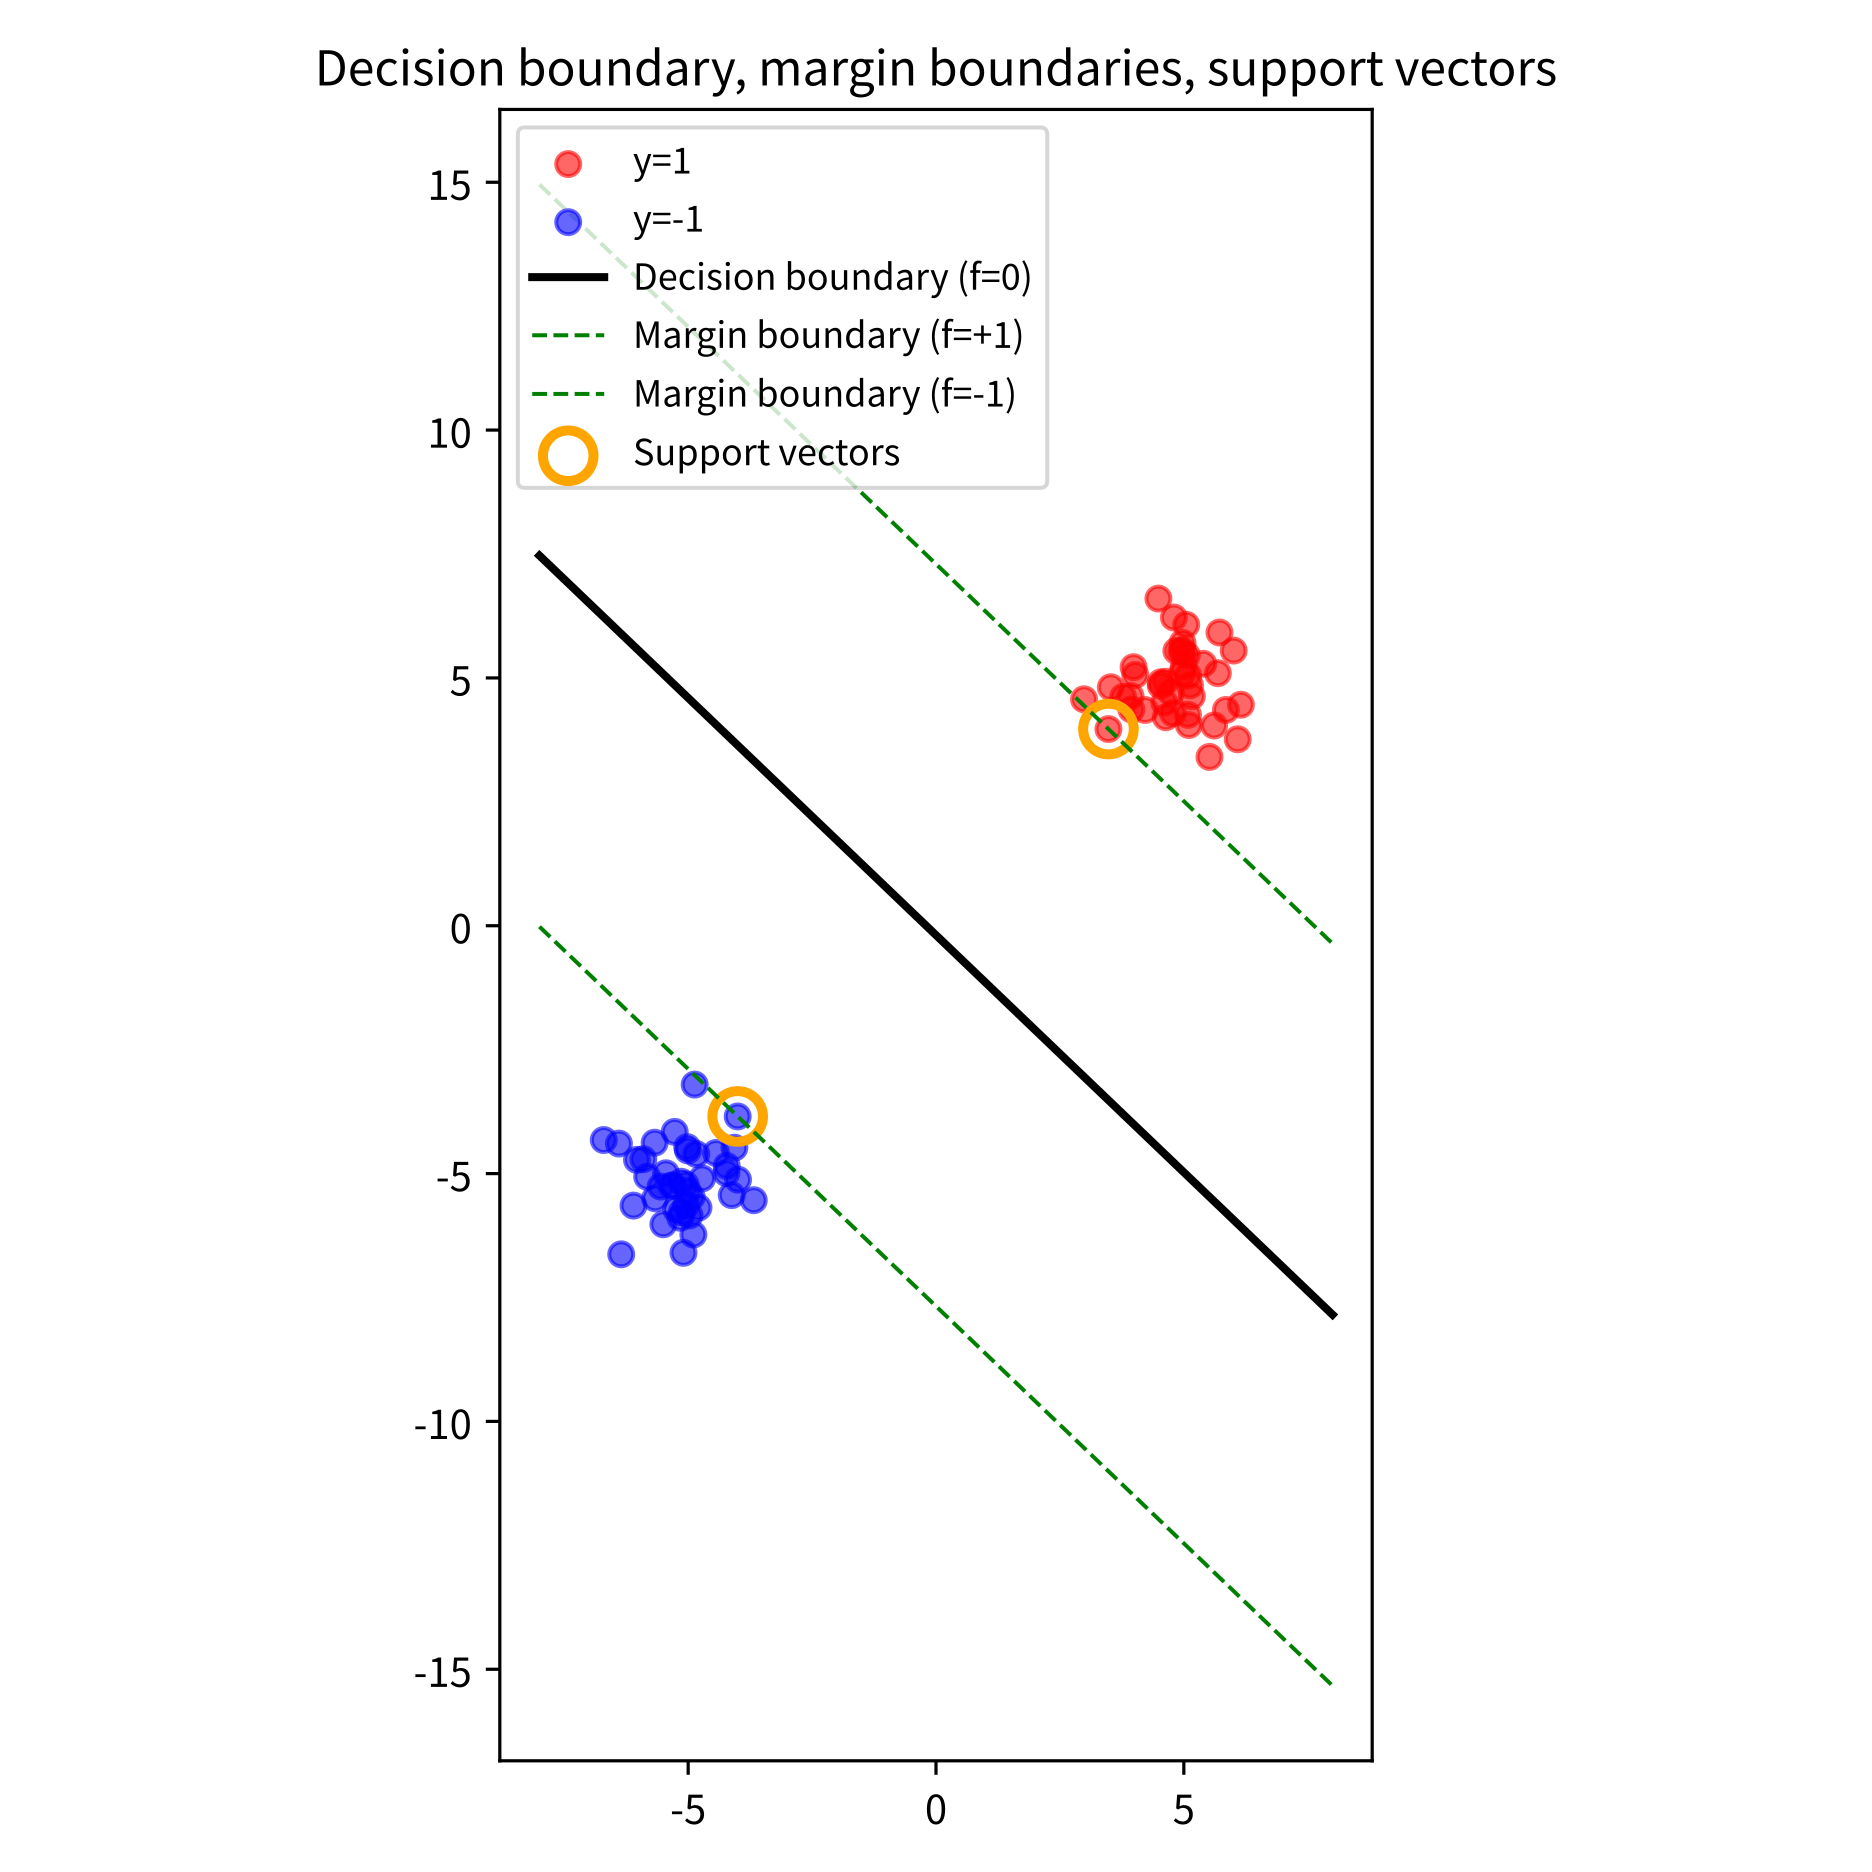
\includegraphics[width=\linewidth]{ch05_1_svm_margin.png}
    \end{column}
    \begin{column}{0.44\textwidth}
      \small
      \begin{itemize}
        \item \kb{마진 경계선}(f=$\pm1$)은 결정 경계(f=0)와 \textbf{평행}.
        \item 두 마진 경계선 \textbf{사이에 데이터가 없음}.
        \item 오렌지 원: \kb{서포트 벡터}만 마진 경계 위에.
      \end{itemize}
      \vskip0.5em
      {\footnotesize 코드의 마지막 두 줄이 경계에서 서포트 벡터까지의
      실제 거리 $= 1/\|w\|$임을 직접 재서, 마진 공식 $2/\|w\|$가
      추상적 수식이 아니라 \textbf{실제 거리}임을 확인.}
    \end{column}
  \end{columns}
\end{frame}

\begin{frame}{노트북에서 확인하는 핵심 세 가지}
  \begin{enumerate}
    \item \kb{마진 경계선이 경계에 평행}하며, 그 사이가 ``마진'' —
      데이터는 마진 경계선 바깥에만 있다.
    \item \kb{서포트 벡터는 마진 경계선 위에만 있다} —
      그 밖의 점은 지워도 $w, b$가 변하지 않는다.
    \item \kb{마진 너비 $2/\|w\|$가 실제 거리와 일치} —
      경계에서 서포트 벡터까지의 유클리드 거리가 정확히
      $1/\|w\|$인지 직접 재본다.
  \end{enumerate}
  \vskip0.6em
  {\footnotesize 실습 노트북: notebooks/ml1/chapter05\_1\_svm\_margin.ipynb —
  병진(shift) 실험과 ``서포트 벡터 아닌 점 이동'' 실험까지 포함.}
\end{frame}

\begin{frame}{역사: ``마진''이라는 생각의 기원}
  \begin{itemize}
    \item 1960년대, \kb{Vapnik}은 모델의 복잡도를 수치화하는
      \kb{VC 차원}(Vapnik--Chervonenkis dimension, Vapnik \& Chervonenkis 1971)을
      만들었다.
    \item 이진 분류기의 VC 차원 = ``그 모델이 \textbf{모든 라벨링에}
      완벽히 맞힐 수 있는 데이터의 최대 개수'' — 모델의 \textbf{용량} 척도.
    \item 바프닉의 핵심 통찰:
    \begin{itemize}
      \item 용량이 작을수록(모델이 단순할수록) 과적합 위험이 줄어든다.
      \item \textbf{마진을 최대화하는 것은 이 용량을 자동으로 제한}하는
        방법 — 마진이 넓으면 경계 근처의 점을 뒤집으려면
        $w$를 꽤 크게 돌려야 하므로,
        ``기울기 변화의 비용'' $\frac12\|w\|^2$가
        모델 복잡도를 자연스럽게 규제한다.
    \end{itemize}
    \item 1990년대 중반, \kb{Cortès}와 함께 SVM을 완성하며
      ``마진 최대화''는 독립된 원리로 자리 잡았다.
  \end{itemize}
  \vskip0.4em
  {\footnotesize 로지스틱회귀=``확률'', GDA/나이브베이즈=``생성 과정'',
  SVM=``경계의 안전 마진'' — 목적지가 다르면 얻는 성질도 다르다.}
\end{frame}

\begin{frame}{자주 하는 실수: ``클러스터를 넓게 벌린다'')}
  \kq{``마진 최대화'' $\neq$ ``두 클래스의 평균 위치를 멀리 벌린다''.}
  \begin{itemize}
    \item 결정 경계는 \textbf{오직} $(3,3)$과 $(-3,-3)$ 두 점의
      위치에만 의존한다.
    \item $(4,3)$을 $(100,100)$으로 옮겨도(다른 5개 점은 그대로)
      다시 학습시킨 $w, b$는 \textbf{소수점까지 완전히 동일} —
      $(100,100)$은 애초에 서포트 벡터가 아니었기 때문.
    \item ``마진 최대화''는 전체 데이터의 평균적 퍼짐이 아니라,
      \textbf{경계에 가장 가까운 소수의 점(서포트 벡터)까지의 거리}
     만을 기준으로 삼는다.
  \end{itemize}
  \vskip0.5em
  \begin{block}{실습으로 재현}
    서포트 벡터 \textbf{아닌} 점을 가장 바깥으로 크게 이동시켜
    재학습하면 $w, b$가 소수점 아래까지 동일.
    반대로 로지스틱회귀는 같은 점 이동에도 $w$가 달라진다 —
    ``모든 점이 손실에 기여''하는 모델에서는 멀리 있는 점도
    (비록 작게라도) 기울기에 영향을 주므로.
  \end{block}
\end{frame}

\begin{frame}{자주 묻는 질문 (1/2)}
  \textbf{Q. 서포트 벡터가 몇 개나 되나요?}
  \begin{itemize}
    \item 데이터에 따라 다르지만 보통 전체 중 \textbf{소수}
      (위 예시: 6개 중 2개).
    \item 개수가 적을수록 ``기억해야 할 정보''가 적다 —
      예측 시에도 전체가 아닌 \textbf{서포트 벡터와만} 비교하면
      된다(kNN은 전체 데이터를 다 봐야 하는 것과 대조).
  \end{itemize}
  \vskip0.5em
  \textbf{Q. $w^\top x+b$의 값이 ``1''이든 ``0.5''든 뭐가 다른가요?}
  \begin{itemize}
    \item 숫자 ``1'' 자체는 아무 의미 없다 —
      $(w,b)$를 $k$배로 쓰면 $w^\top x+b$도 $k$배가 된다.
    \item 중요한 것은 \textbf{비율}: 제약이 기능적 마진을 ``1로 고정''하는
      자물쇠 역할을 하고, 그 고정이 있어야
      $\frac{2}{\|w\|}$가 스케일에 무관한 실제 거리가 된다.
    \item 제약을 $\ge 0.5$로 쓰면 $w$가 정확히 2배(경계 동일),
      마진 $2/\|w\|$는 절반 — \textbf{결론은 결국 동일}.
  \end{itemize}
\end{frame}

\begin{frame}{자주 묻는 질문 (2/2)}
  \textbf{Q. 라벨을 왜 굳이 $-1/+1$로 바꾸나요?}
  \begin{itemize}
    \item $y^{(i)}(w^\top x^{(i)}+b)$ \textbf{하나의 식}으로
      ``올바른 클래스 쪽에 있는가''와 ``얼마나 여유 있게 있는가''를
      동시에 표현하기 위한 \textbf{표기상의 편의}.
    \item $y=\pm1$이면 ``곱이 클수록 좋다''는 하나의 부등식으로 통일 —
      $0/1$ 라벨이었다면 클래스마다 부등호 방향이 다른 두 식을
      따로 다뤄야 했다.
  \end{itemize}
  \vskip0.5em
  \textbf{Q. 로지스틱회귀와 같은 $w^\top x+b=0$인데, 뭐가 다른가요?}
  \begin{itemize}
    \item \textbf{어떤} 경계를 뽑을지가 다르다:
      로지스틱회귀는 \textbf{모든 점}이 손실에 기여해 분포 전체에 민감
      (매끄러운 경계), SVM은 마진 바깥 점의 손실이 정확히 0이라
      오직 서포트 벡터만 경계를 결정(각진 경계).
    \item \textbf{이상치 견고성}: 이상치가 서포트 벡터가 안 되는 한
      SVM은 무시; 로지스틱회귀는 아무리 멀어도 아주 작은 기울기로
      손실에 영향 — 서로 다른 트레이드오프.
  \end{itemize}
\end{frame}

% =====================================================================
\section{5.2 소프트 마진: 완벽히 나뉘지 않는 데이터}

\begin{frame}{도입: 하드 마진의 치명적인 전제}
  \begin{itemize}
    \item 5.1절 하드 마진: 제약 $y^{(i)}(w^\top x^{(i)}+b)\ge 1$ 아래
      $\|w\|$ 최소화. 쌍대 문제, 서포트 벡터, $2/\|w\|$ 공식 등
      예쁜 성질을 다 갖췄다.
    \item 그런데 \textbf{치명적인 전제}: \kb{데이터가 완벽히 선형분리 가능}.
  \end{itemize}
  \vskip0.5em
  실전 데이터는 노이즈 때문에 이 가정을 거의 만족하지 못한다:
  \begin{itemize}
    \item \kb{라벨링 오류} — 의사가 진단을 틀렸거나,
      스팸 필터 학습용 메일에 사람이 틀린 태그를 붙인 경우
    \item \kb{측정 오류} — 센서 오차
    \item \kb{모호한 경계 사례} — 도메인 밖의 데이터
  \end{itemize}
  \vskip0.4em
  \begin{block}{문제의 심각성}
    어떤 $(w,b)$로도 제약을 모두 만족 못 하면(불일치, infeasible)
    이차계획을 풀 수 없다 — 하드 마진 SVM은 \textbf{라벨 오류
    단 하나만 있어도 해 자체가 존재하지 않는} 모델. 그대로 실전에
    쓸 수 없다.
  \end{block}
\end{frame}

\begin{frame}{소프트 마진: 위반을 허용하는 법}
  고법의 핵심은 한 줄이면 충분하다:
  \begin{center}
  ``제약을 만족 못 하면, \textbf{얼마만큼 못 했는지 재서 벌을}
  부리고, 벌의 크기는 \textbf{하이퍼파라미터로} 조절한다.''
  \end{center}
  \vskip0.6em
  \begin{itemize}
    \item 각 데이터마다 위반을 어느 정도 허용하는
      \kb{여유 변수}(slack variable) $\xi^{(i)} \ge 0$:
      \[
      y^{(i)}\bigl(w^\top x^{(i)}+b\bigr) \ge 1 - \xi^{(i)}
      \]
    \item $\xi^{(i)}$는 ``몇 만큼까지 마진 제약을 무시할 수 있는가''의
      \textbf{권한}.
  \end{itemize}
  \vskip0.4em
  \small
  \begin{tabular}{@{}ll@{}}
    \toprule
    $\xi^{(i)}$의 값 & 의미 \\
    \midrule
    $0$ & 5.1절 제약과 정확히 같음 \\
    $0.5$ & 마진 경계 안쪽으로 0.5쯤 들어와도 괜찮다 (정답, 마진 위반) \\
    $1$ & 결정 경계(마진 0) 위에 있어도 괜찮다 \\
    $>1$ & \textbf{경계 너머(반대쪽 영역)}로 넘어가도 되는 허락 \\
    \bottomrule
  \end{tabular}
  \normalsize\vskip0.3em
  하나의 수 $\xi$가 ``정답인데 마진 안''에서 ``오분류''까지를
  \textbf{연속적으로} 표현한다.
\end{frame}

\begin{frame}{목적함수: 마진 최대화 vs 위반 최소화}
  \begin{itemize}
    \item ``마진을 최대화하고 싶다''($\|w\|$ 최소화)와
      ``위반을 최소화하고 싶다''($\sum\xi$ 최소화)의 트레이드오프:
      \[
      J(w,b) = \frac{1}{2}\|w\|^2 + C\sum_{i=1}^{m} \xi^{(i)}
      \]
    \item \kb{힌지 손실}(hinge loss)로 다시 쓸 수 있다 —
      $\max(0,\cdot)$이 $\xi^{(i)}$의 최소값을 자동으로 계산해주기
      때문:
      \[
      J(w,b) = \frac{1}{2}\|w\|^2
      + C\sum_{i=1}^{m} \max\bigl(0,\ 1-y^{(i)}(w^\top x^{(i)}+b)\bigr)
      \]
  \end{itemize}
  \vskip0.5em
  \begin{block}{$C$: 이 절의 유일한 손잡이}
    $C$가 \textbf{크면} 위반에 더 엄격 $\Rightarrow$ 라벨에 충실
    (과적합 위험).
    $C$가 \textbf{작으면} 마진을 넓게 잡는 대신 위반을 더 허용
    (과소적합 위험).
    6장의 정규화 세기 조절과 \textbf{정확히 같은 종류}의 트레이드오프.
  \end{block}
\end{frame}

\begin{frame}{``힌지''의 모양과 $C$라는 손잡이}
  $f = y^{(i)}(w^\top x^{(i)}+b)$를 자변수로 하면
  $L(f) = \max(0, 1-f)$:
  \begin{itemize}
    \item $f < 1$: 기울기 $-1$로 \textbf{선형 증가}
    \item $f \ge 1$: \textbf{정확히 0으로 꺾여} 평평해짐
      ($f=1$에서 ``접힌''(kink) 삼각형 — 이름의 유래)
    \item 힌지: 충분히 맞히면 \textbf{아예} 손실 0 / 기여 0.
      교차 엔트로피: 아무리 맞혀도 $1-\sigma(f)>0$ — 기여가
      \textbf{절대 0이 안 됨}.
  \end{itemize}
  \vskip0.4em
  \begin{block}{$C$: ``이상치 용인도''를 조절하는 손잡이}
    $C$ \textbf{크면} ``위반을 무겁게 벌하라'' = \textbf{라벨에
    충실하게} 경계를 맞추라(과적합 위험).
    $C$ \textbf{작으면} ``라벨이 틀려도 괜찮으니 대신 마진을 넓게''
    (과소적합 위험).
    \vskip0.3em
    2장의 \textbf{학습률}, 4장의 \textbf{$k$}와 함께 모델의
    ``\textbf{데이터 충실도 vs 단순함}''을 조절.
    5.3절 RBF에서는 여기에 경계 \textbf{구부러짐}을 조절하는
    $\gamma$가 더 생긴다.
  \end{block}
  \vskip0.3em
  {\footnotesize 이 절의 실험엔 이상치를 \textbf{의도적으로}
  넣는다 — 이상치가 있는 곳에서 $C$가 무엇을 하는지 보면,
  없는 곳에서 $C$의 ``극한 한계 행동''이 직관적으로 보인다.}
\end{frame}

\begin{frame}{손으로 한 번: 힌지 손실과 $C$의 효과}
  대칭 데이터에 이상치 두 개 추가: 정상 $(3,3){\to}+1$,
  $(-3,-3){\to}-1$ + 반대쪽 영역에 잘못 놓인
  $(2,-3){\to}+1$, $(-2,3){\to}-1$.
  후보 경계 $w=(0.2,0.2)$, $b=0$ 에 대해:
  \small
  \begin{tabular}{@{}lcc@{}}
    \toprule
    점 & $y^{(i)}(w^\top x^{(i)}+b)$ & 힌지 손실 \\
    \midrule
    $(3,3),\,+1$ & $0.2\cdot3+0.2\cdot3=1.2$ & $\max(0,1-1.2)=0$ \\
    $(-3,-3),\,-1$ & $(-1)(-0.6-0.6)=1.2$ & $0$ \\
    $(2,-3),\,+1$ & $0.2\cdot2+0.2(-3)=-0.2$ & $\max(0,1.2)=1.2$ \\
    $(-2,3),\,-1$ & $(-1)(-0.4+0.6)=-0.2$ & $1.2$ \\
    \bottomrule
  \end{tabular}
  \normalsize\vskip0.4em
  전체 목적함수: $\frac12\|w\|^2=0.04$, $\sum\xi^{(i)}=2.4$ 이므로
  \[
  C{=}0.1: J=0.04+0.1\times2.4=0.28
  \qquad
  C{=}10: J=0.04+10\times2.4=24.04
  \]
  \vskip0.3em
  \begin{itemize}
    \item 정상 점: 마진을 넉넉히 만족 $\Rightarrow$ 손실 0;
      이상치: 반대쪽 영역에 있어서 손실 1.2씩.
    \item 같은 $(w,b)$인데 $C$가 커질수록 이상치 손실이
      \textbf{완전히 지배} — $C=10$은 경계를 크게 \textbf{구부리거나}
      촘촘히 맞추려 하고, $C=0.1$은 마진을 넓게 유지하고 이상치는
      ``\textbf{어쩔 수 없는 노이즈}''로 용인.
  \end{itemize}
\end{frame}

\begin{frame}{손으로 한 번: 힌지 손실의 그래디언트}
  $f = y^{(i)}(w^\top x^{(i)}+b)$, $L = \max(0, 1-f)$ 의 그래디언트:
  \[
  \frac{\partial L}{\partial w} =
  \begin{cases}
  -y^{(i)}x^{(i)} & \text{if } f < 1 \quad (\text{마진 위반})\\
  0 & \text{if } f \ge 1 \quad (\text{마진 만족})
  \end{cases}
  \qquad
  \frac{\partial L}{\partial b} =
  \begin{cases}
  -y^{(i)} & \text{if } f < 1\\
  0 & \text{if } f \ge 1
  \end{cases}
  \]
  \vskip0.4em
  \begin{itemize}
    \item 마진을 만족하는 점의 기여는 \textbf{정확히 0}.
    \item 로지스틱회귀에서는 아무리 잘 맞혀도 $1-\sigma(f)>0$이라
      모든 점이 계속 기울기에 기여했지만, 힌지 손실은
      ``충분히 맞힌'' 점의 기여가 \textbf{완전히} 사라진다.
    \item 이 차이가 \kb{서포트 벡터} 개념을 가능하게 한다.
  \end{itemize}
\end{frame}

\begin{frame}{학습 궤적으로 확인: 대칭 데이터}
  $hinge\_loss\_gradient\_descent$를 $C=1.0,\ \alpha=0.01$로
  5.1절 대칭 데이터에 적용하면 ($b$는 처음부터 끝까지 정확히 0):
  \small
  \begin{tabular}{@{}ccc@{}}
    \toprule
    에폭 & $w_1\ (=w_2)$ & $b$ \\
    \midrule
    1 & 0.0333 & 0.0000 \\
    10 & 0.1750 & 0.0000 \\
    100 & 0.1719 & 0.0000 \\
    2000 & 0.1735 & 0.0000 \\
    \bottomrule
  \end{tabular}
  \normalsize\vskip0.5em
  \begin{itemize}
    \item 몇십 에폭 만에 $w\approx0.17$로 수렴 — 5.1절의 정확해
      $(1/6,1/6)\approx(0.167,0.167)$에 잘 붙는다.
    \item 정확히 0.1667이 아니라 0.1735에 머무는 것은, full-batch
      경사하강이 힌지 손실의 ``꺾임''($f=1$에서 미분 불가) 때문에
      최적해 근처에서 \textbf{약간 진동}하며 2000 에폭 만에
      완전히 가라앉지 않기 때문.
    \item 대칭 데이터: 두 클래스의 위반 패턴이 완전히 대칭 $\Rightarrow$
      $b$의 그래디언트가 항상 상쇄되어 0.
      \textbf{실제 데이터는 대칭이 아니므로} $b$가 0에서 벗어나
      경계의 위치를 결정.
  \end{itemize}
\end{frame}

\begin{frame}{소프트 마진의 세 가지 영역}
  하드 마진에선 ``마진 경계 $f=\pm1$ 안에 데이터가 없다''가
  제약 그 자체. 소프트 마진에선 각 데이터가 $\xi^{(i)}$의 크기에
  따라 세 영역 중 하나:
  \small
  \begin{tabular}{@{}p{3.1cm}p{3.4cm}p{2.4cm}p{3.2cm}@{}}
    \toprule
    영역 & 조건 & $\xi^{(i)}=\max(0,1-f)$ & 의미 \\
    \midrule
    ① 마진 바깥 정답 & $f \ge 1$ & $0$ & 손실 0, 경계에 영향
      없음(서포트 벡터 아님) \\
    ② 마진 안 정답 & $0 < f < 1$ & $1-f$ & 마진 일부 침범 —
      경계에 기여(서포트 벡터) \\
    ③ 경계 너머 & $f \le 0$ & $\ge 1$ & 오분류 상태 — 손실 1 이상,
      가장 강하게 기여 \\
    \bottomrule
  \end{tabular}
  \normalsize\vskip0.5em
  \begin{itemize}
    \item \kb{$\xi$의 크기가 ``문제의 심각도''를 연속적으로 재줌}.
    \item $f=0.9$ (②): $\xi=0.1$으로 거의 정상.
      $f=-0.2$ (③): $\xi=1.2$로 12배 비싼 오류.
    \item 경계를 넘으면 손실이 1을 기점으로 기울기가 바뀌는 것이
      아니라, \textbf{기울기는 $-1$으로 동일}한 채 절대값만 커진다.
    \item 힌지 손실은 ``경계 너머로 멀리''를 ``경계 위에''보다
      특별히 크게 벌하지 않는다 — 로지스틱회귀의 $-\log\sigma$가
      지수적으로 벌하는 것과 대비.
  \end{itemize}
\end{frame}

\begin{frame}[fragile]{실습: 소프트 마진의 세 영역을 눈으로 보자}
  \begin{lstlisting}
import numpy as np
import matplotlib.pyplot as plt
from sklearn.svm import SVC

# 5.1절 대각선 클러스터 + 이상치 두 개
rng = np.random.default_rng(7)
X = np.vstack([rng.normal([5, 5], 0.8, (40, 2)),
               rng.normal([-5, -5], 0.8, (40, 2)),
               np.array([[2.0, -3.0], [-2.0, 3.0]])])
y = np.r_[np.ones(40), -np.ones(40), [1.0, -1.0]]

clf = SVC(kernel="linear", C=1.0).fit(X, y)
wc, bc = clf.coef_[0], clf.intercept_[0]
sv = X[clf.support_]                          # 서포트 벡터만
outs = X[80:82]                               # 이상치 두 개

x1 = np.linspace(-8, 8, 100)
f_line = lambda c: (-wc[0]*x1 - bc + c) / wc[1]   # f = c 의 직선

fig, ax = plt.subplots(figsize=(6.5, 6.5))
for lbl, col in [(1, "red"), (-1, "blue")]:
    ax.scatter(X[y == lbl, 0], X[y == lbl, 1], color=col,
               alpha=0.6, label=f"y={lbl}")
ax.plot(x1, f_line(0),  "k",   lw=2,  label="결정 경계 (f=0)")
ax.plot(x1, f_line(1),  "g--", lw=1, label="마진 경계 (f=+1)")
ax.plot(x1, f_line(-1), "g--", lw=1, label="마진 경계 (f=-1)")
ax.scatter(sv[:, 0], sv[:, 1], s=160, facecolors="none",
           edgecolors="orange", lw=2.5, label="서포트 벡터")
ax.scatter(outs[:, 0], outs[:, 1], s=260, marker="*",
           facecolors="white", edgecolors="red", lw=1.5, label="이상치")
ax.set_aspect("equal"); ax.legend(loc="upper left", fontsize=9)
ax.set_title("소프트 마진: 이상치가 마진 안/너머로 허용됨 (C=1)")
plt.show()

# 이상치가 어느 영역(②/③)에 빠졌는지 직접 계산
for i in [80, 81]:
    m = y[i] * (wc @ X[i] + bc)
    print(f"이상치 {tuple(X[i])}: f={m:+.3f} -> xi={max(0.0,1-m):.3f}, "
          f"{'서포트 벡터' if i in clf.support_ else '아님'}")
print(f"서포트 벡터 {len(sv)}개 / 전체 {len(X)}개,  마진 2/||w|| = {2/np.linalg.norm(wc):.3f}")
\end{lstlisting}
\end{frame}

\begin{frame}{그림으로 읽기: 하드 마진과의 세 가지 차이}
  \begin{columns}[T]
    \begin{column}{0.52\textwidth}
      \centering
      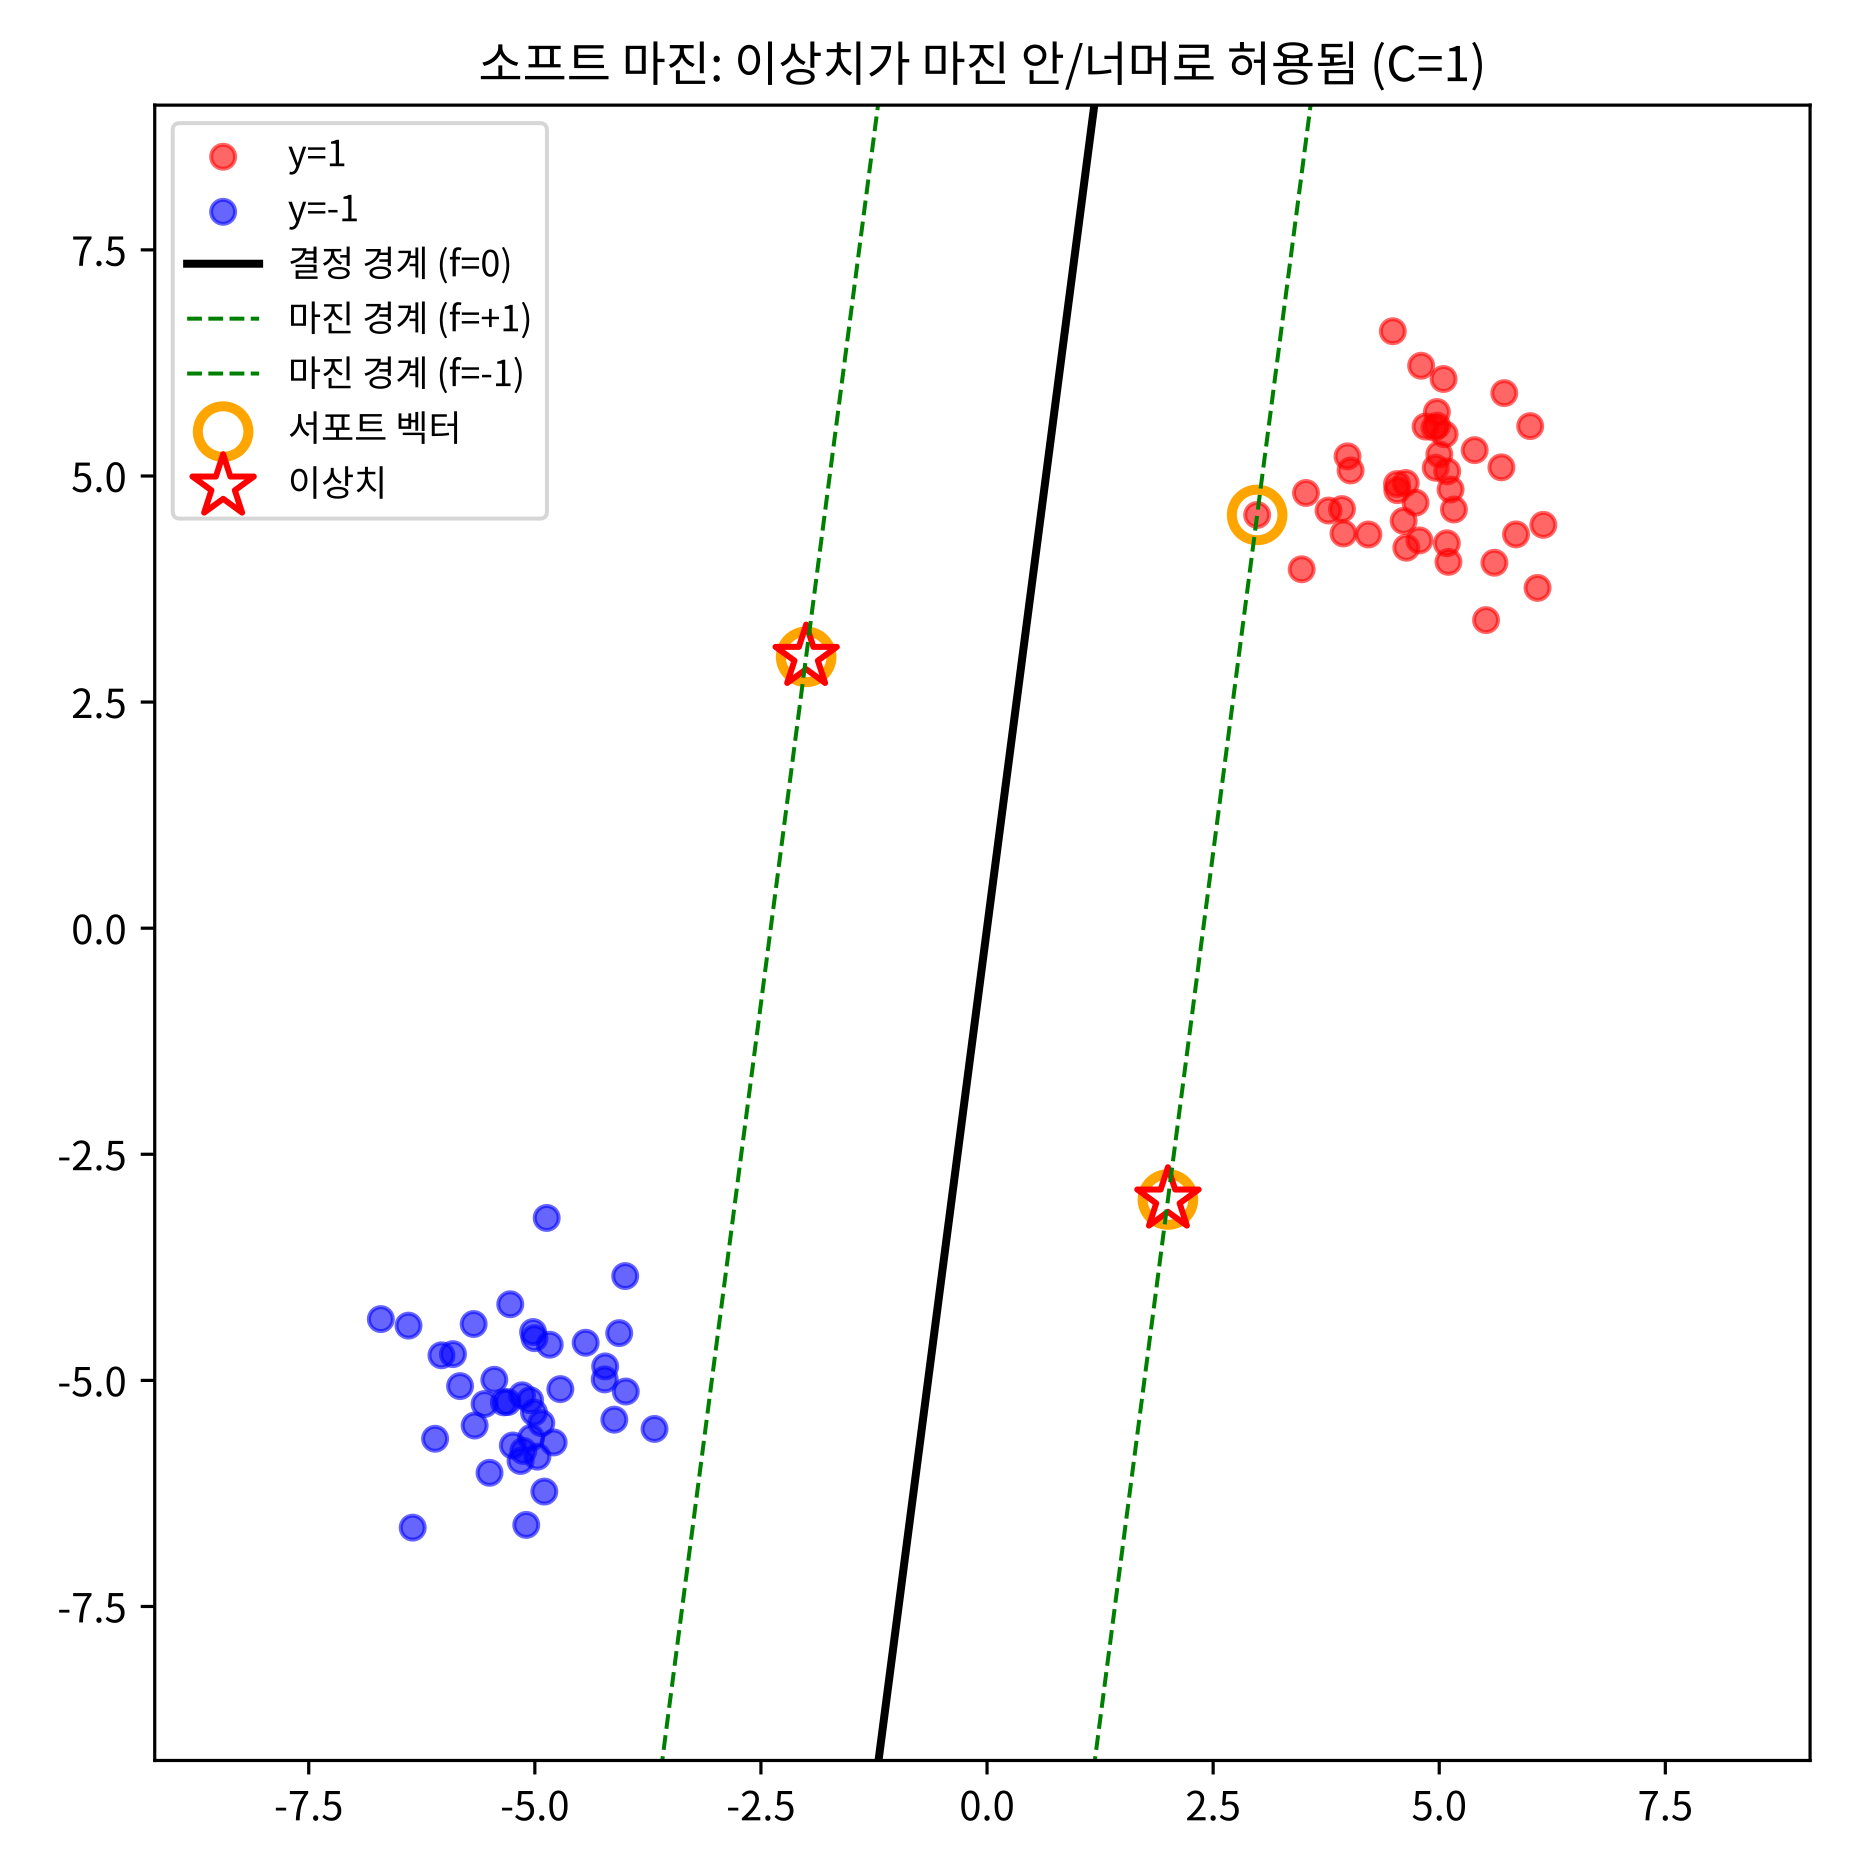
\includegraphics[width=\linewidth]{ch05_2_soft_margin.png}
    \end{column}
    \begin{column}{0.44\textwidth}
      \small
      \begin{enumerate}
        \item \kb{마진 경계 안에 데이터가 들어와 있다} — 5.1절에선
          $f=\pm1$ 사이에 아무 점도 없었지만, 여기서는 이상치가
          마진 안(또는 경계 너머)에 있다. 허용된 것이지 결함이
          아니다.
        \item \kb{서포트 벡터의 위치가 바뀌었다} — 이상치 두 개가
          서포트 벡터에 포함(코드 출력: 인덱스 80, 81 모두
          $f=+1.000$, $\xi=0$). 이상치를 ``받아안으려다''
          마진 경계 위에 정확히 올려놓은 것.
        \item \kb{마진이 5.1절보다 좁아졌다} — $2/\|w\|$가
          $\approx8.5$보다 작다. 이상치를 받으려면 $\|w\|$가 커져
          마진이 좁아진다 — $C$가 조절하는 트레이드오프의 단면.
      \end{enumerate}
      \vskip0.4em
      {\footnotesize 이상치는 ``완벽한 이상치''(다른 클래스 근처)가
      아니라 \textbf{경계 쪽 클러스터 사이에 놓인} 점. $C=1$에선
      어느 영역(② 또는 ③)에 빠지는지 예측해라.}
    \end{column}
  \end{columns}
\end{frame}

\begin{frame}[fragile]{실습: $C$ 스윕 — 이상치를 무시할지 받아안을지}
  \begin{lstlisting}
import numpy as np
from sklearn.svm import SVC

# 클러스터 ±(2.5,2.5) 스프레드 0.6, 각 40개 + 이상치 (-1.6,0.8)
rng = np.random.default_rng(21)
n = 40
X = np.vstack([rng.normal([2.5, 2.5], 0.6, (n, 2)),
               rng.normal([-2.5, -2.5], 0.6, (n, 2)),
               np.array([[-1.6, 0.8]])])
y = np.r_[np.ones(n), -np.ones(n), [1.0]]

# 같은 데이터를 C = 0.01, 0.1, 1, 10, 100 으로 학습
Cs = [0.01, 0.1, 1.0, 10.0, 100.0]
print(f"{'C':>7s} {'마진 2/||w||':>12s} {'b/||w||':>8s} "
      f"{'n_SV':>5s} {'이상치 f':>10s} {'정상점 오분류':>12s}")
for C in Cs:
    clf = SVC(kernel="linear", C=C).fit(X, y)
    wc, bc = clf.coef_[0], clf.intercept_[0]
    om = y[-1] * (wc @ X[-1] + bc)     # 이상치의 기능적 마진
    mis = (clf.predict(X[:-1]) != y[:-1]).sum()
    print(f"{C:7.2f} {2/np.linalg.norm(wc):12.3f} "
          f"{bc/np.linalg.norm(wc):+8.3f} {len(clf.support_):5d} "
          f"{om:10.3f} {mis:12d}")
\end{lstlisting}
\end{frame}

\begin{frame}{$C$ 스윕 결과}
  \small
  \begin{tabular}{@{}ccccc@{}}
    \toprule
    $C$ & 마진 $2/\|w\|$ & $b/\|w\|$ & 서포트 벡터 수 & 이상치 $f$ \\
    \midrule
    0.01 & 6.01 & $+0.02$ & 14 & $-0.16$ \\
    0.1  & 4.61 & $+0.23$ & 5  & $+0.08$ \\
    1.0  & 2.30 & $+0.65$ & 2  & $+1.00$ \\
    10.0 & 2.30 & $+0.65$ & 2  & $+1.00$ \\
    100.0& 2.30 & $+0.65$ & 2  & $+1.00$ \\
    \bottomrule
  \end{tabular}
  \normalsize\vskip0.5em
  \begin{itemize}
    \item \kb{$C=0.01$ (이상치 무시)}: 마진 가장 넓음(6.01), 이상치
      $f=-0.16$로 \textbf{결정 경계 너머}(③, 오분류). SV 14개 —
      원래 두 클러스터만 보고 ``정직한'' 경계, 대가로 이상치를
      버린다.
    \item \kb{$C=0.1$ (일부 수용)}: 마진 4.61로 좁혀지고, 이상치
      $f=+0.08$로 \textbf{경계 안}으로(②, 마진 위반). SV 5개.
    \item \kb{$C\ge1$ (완전 수용)}: 이상치 $f=1.00$으로
      \textbf{마진 경계 위에}(②의 한계, $\xi=0$). 이상치가 SV가
      되어 경계를 떠받치고, 마진 2.30.
  \end{itemize}
\end{frame}

\begin{frame}{$C$ 스윕: ``지수'' 현상}
  \begin{itemize}
    \item $C=1$에서 이미 이상치를 \textbf{완전히 수용}했으므로
      $C=10, 100$으로 더 올려도 결과(경계·마진·SV)가 \textbf{모두
      동일}.
    \item 이상치가 하나뿐이고 \textbf{그 이상치가 수용되면}
      $C$를 더 올려도 변하지 않는다.
  \end{itemize}
  \vskip0.5em
  \begin{block}{실용적 함의: $C$ 튜닝의 상한선}
    이 ``지수'' 현상은 $C$ 튜닝의 \textbf{실용적 상한선}을 알려준다 —
    검증셋 정확도가 더 이상 변하지 않는 $C$ 이상은
    \textbf{과적합 위험만 키울 뿐}.
  \end{block}
  \vskip0.5em
  \begin{columns}[T]
    \begin{column}{0.52\textwidth}
      \centering
      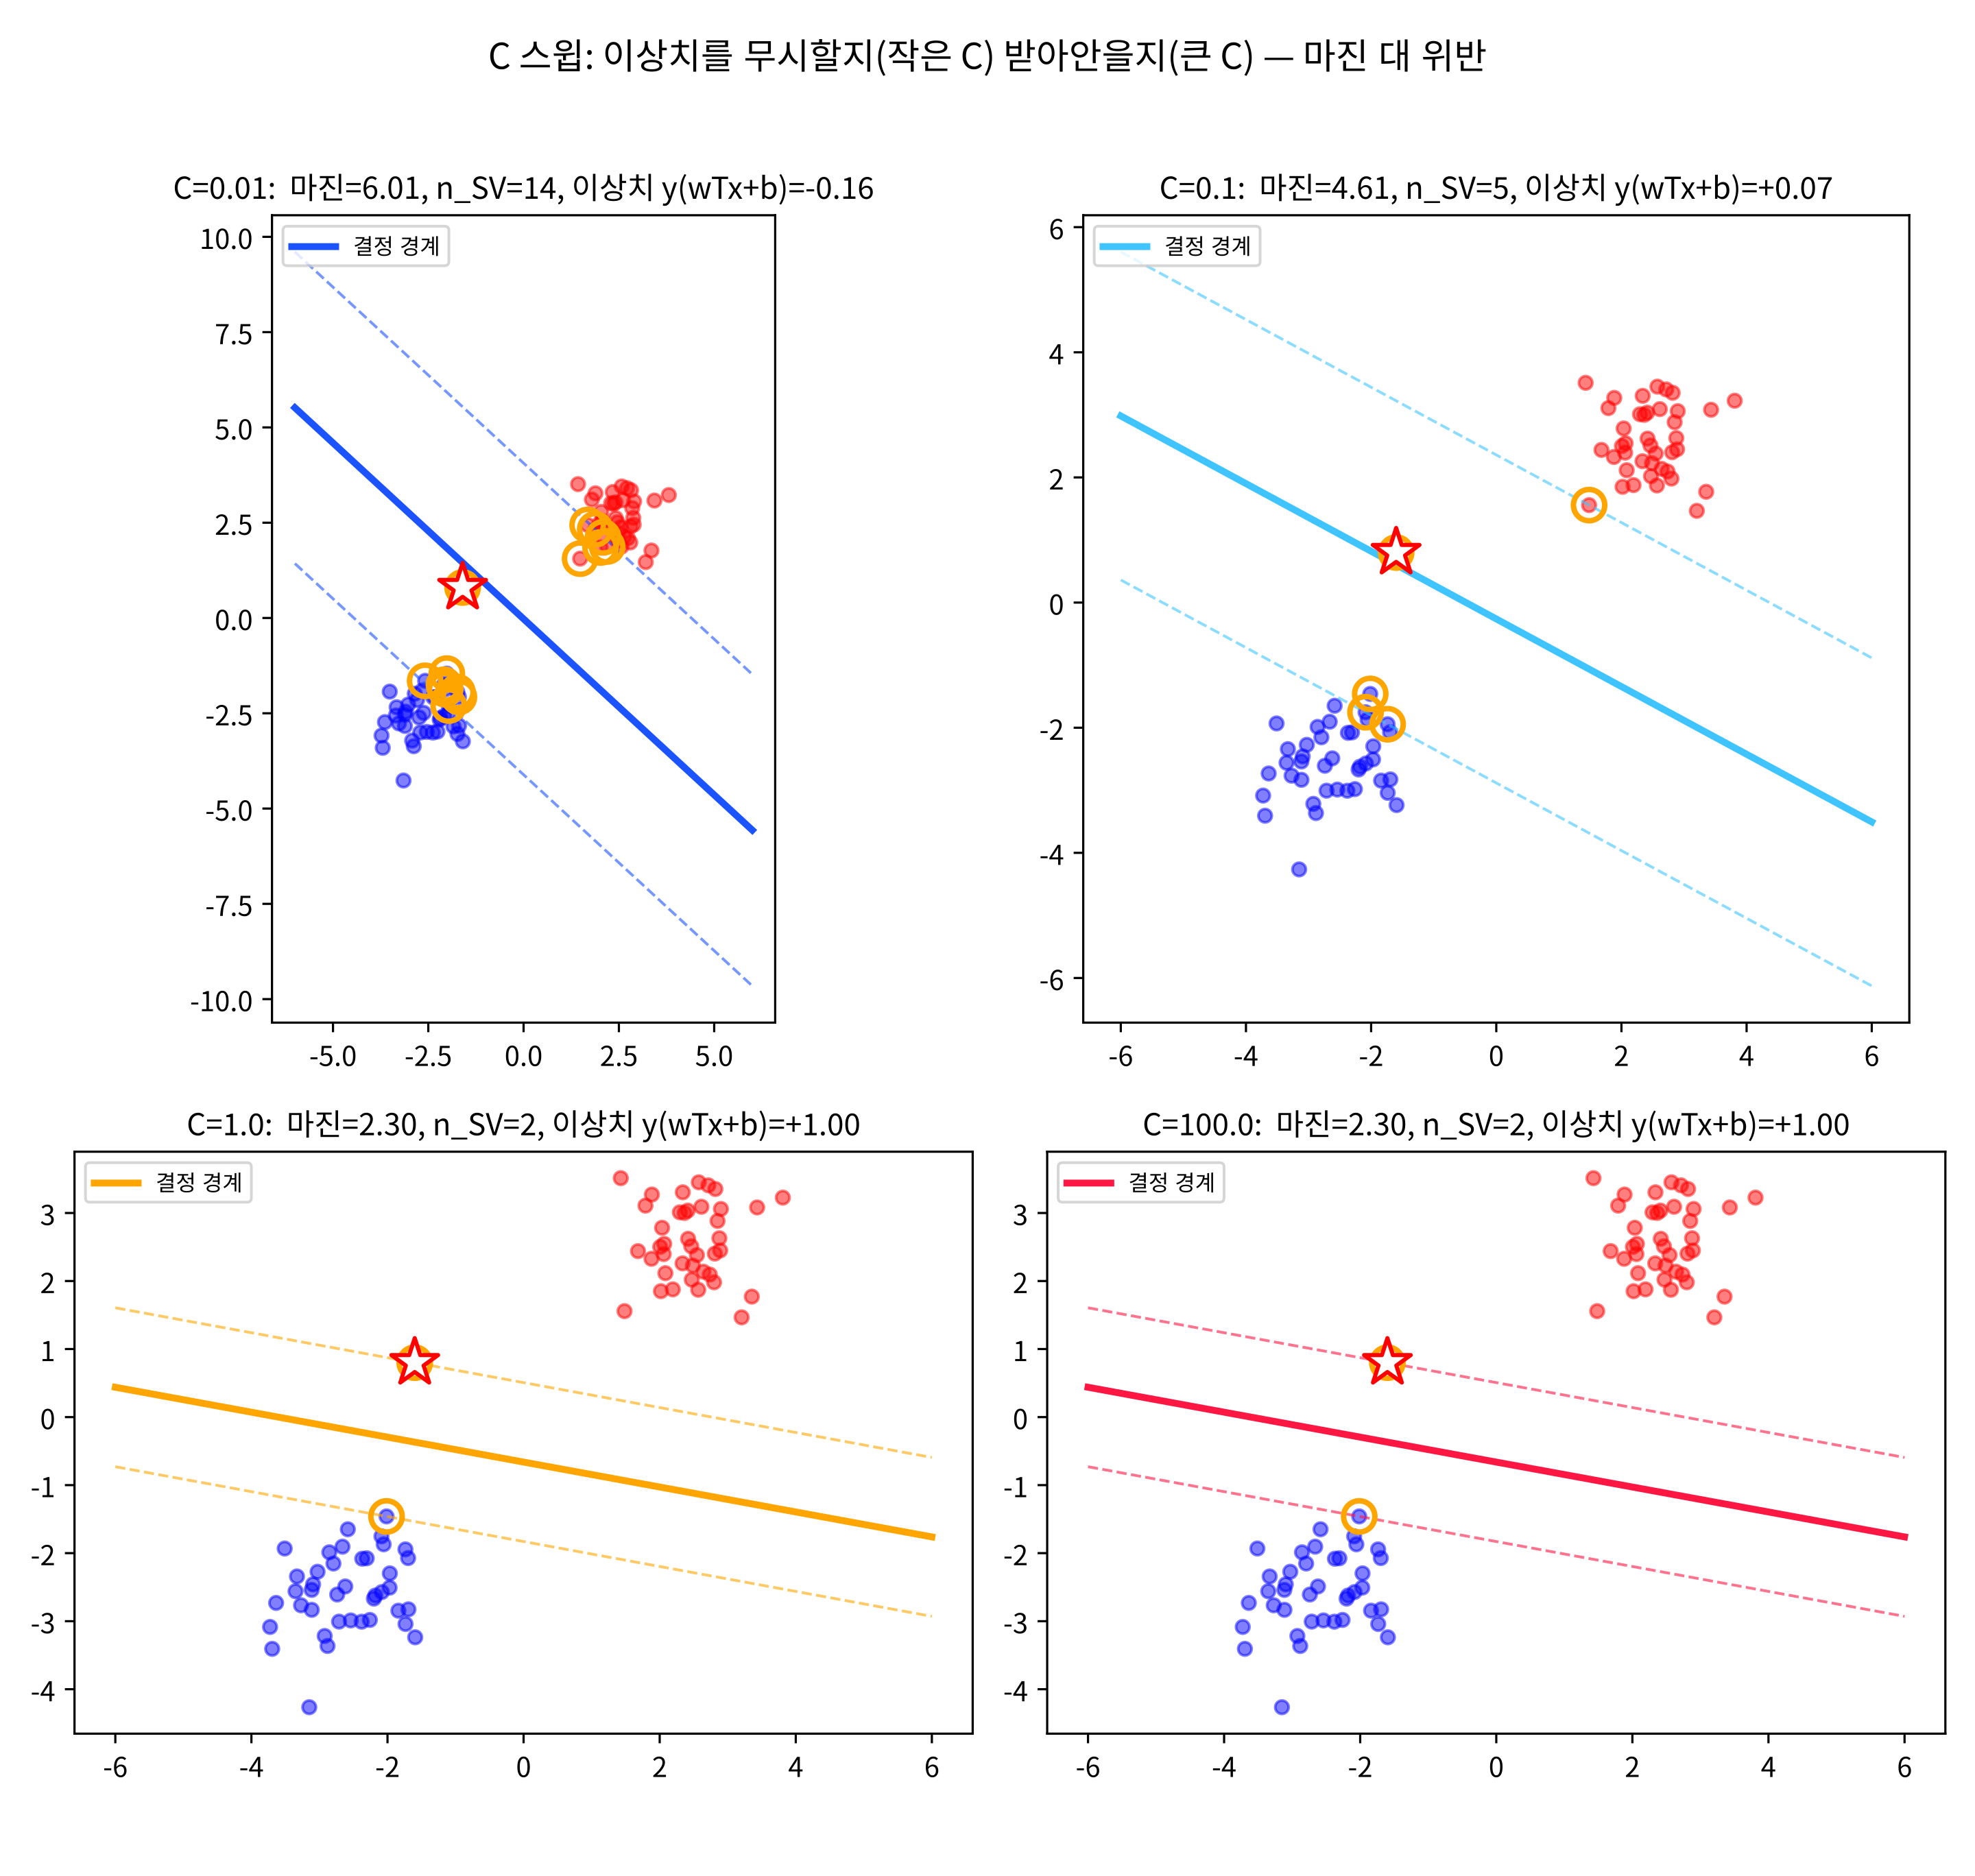
\includegraphics[width=\linewidth]{ch05_2_C_sweep.png}
    \end{column}
    \begin{column}{0.44\textwidth}
      \small
      \begin{itemize}
        \item $C=0.01$: 이상치(빨간 별)가 결정 경계 \textbf{너머}
          (옅은 색 영역)에 남아 있음.
        \item $C=100$: 이상치가 \textbf{마진 경계 위에} 정확히
          놓여 있음.
        \item \textbf{같은 데이터, 다른 $C$ $\Rightarrow$ 다른 경계} —
          $C$가 ``경계의 위치''를 실제로 결정한다는 직접적 증거.
      \end{itemize}
    \end{column}
  \end{columns}
\end{frame}

\begin{frame}[fragile]{라벨 노이즈: $C$가 과적합을 조절하는 방식}
  \begin{itemize}
    \item 실전에서 더 흔한 문제는 \kb{라벨링 오류} — 데이터가 수천
      개면 라벨이 틀린 것 5$\sim$15\% 섞여 있는 것이 \textbf{정상}.
    \item 이상치와의 차이: 라벨 노이즈는 \textbf{경계 근처에 있는}
      점의 라벨이 뒤집혀 있다.
    \item 이 경우 $C$의 역할이 가장 극적으로 드러난다:
      $C$가 클수록 ``모든 라벨에 충실하려'' 틀린 라벨까지 맞춰주려
      경계를 그 오류 쪽으로 끌고 간다.
  \end{itemize}
  \vskip0.5em
  \small
  \textbf{실험 설정}: 클러스터 $\pm(3,3)$ (스프레드 1.5, 각 100개,
  총 200개). $y=+1$ 중 \textbf{경계에 가장 가까운 30개}(15\%)의
  라벨을 $-1$로 뒤집기. 테스트: 같은 분포의 \textbf{깨끗한} 600개.
  \normalsize
  \vskip0.5em
  \begin{lstlisting}
rng2 = np.random.default_rng(5)
n2 = 100
Xn = np.vstack([rng2.normal([3, 3], 1.5, (n2, 2)),
                rng2.normal([-3, -3], 1.5, (n2, 2))])
yn = np.r_[np.ones(n2), -np.ones(n2)]
pos_scores = Xn[:n2].sum(axis=1)      # 경계(원점)에 가까울수록 작음
flip_idx = np.argsort(pos_scores)[:30]  # +1 중 경계 가장 가까운 30개
yn[flip_idx] = -1                     # 라벨 15% 뒤집기
# ... SVC(C)와 LogisticRegression을 각각 fit, train/test score 출력
\end{lstlisting}
\end{frame}

\begin{frame}{라벨 노이즈 결과: 과적합의 교과서적 신호}
  \small
  \begin{tabular}{@{}lccc@{}}
    \toprule
    모델 & train & test & $b/\|w\|$ \\
    \midrule
    SVC $C=0.01$ & 0.865 & \textbf{0.968} & $-1.88$ \\
    SVC $C=0.1$  & 0.995 & 0.877 & $-3.13$ \\
    SVC $C=1.0$  & 0.995 & 0.870 & $-3.22$ \\
    SVC $C=10$   & 0.995 & 0.875 & $-3.17$ \\
    SVC $C=100$  & 1.000 & 0.877 & $-3.13$ \\
    로지스틱회귀 & 0.995 & 0.873 & $-3.17$ \\
    \bottomrule
  \end{tabular}
  \normalsize\vskip0.5em
  \begin{itemize}
    \item \textbf{가장 중요한 숫자}: $C=0.01$의 test $0.968$ —
      train은 0.865로 ``최악''인데 \textbf{test는 가장 높다}.
    \item $C\ge0.1$: train 0.995$\sim$1.000(라벨 오류까지 거의 다
      맞힘)인데 test는 0.87$\sim$0.88로 \textbf{떨어진다}.
    \item 이 패턴(\textbf{train$\uparrow$ test$\downarrow$}) =
      과적합의 교과서적 신호, $C$가 그 \textbf{조절 밸브}.
  \end{itemize}
\end{frame}

\begin{frame}{$b/\|w\|$: 경계가 얼마나 밀렸는가}
  \begin{itemize}
    \item $b/\|w\|$ = 결정 경계의 \textbf{원점에서의 거리}(부호
      포함) — ``경계가 원점(정직한 위치)에서 얼마나 밀렸는가''.
    \item $C=0.01$: $-1.88$ — 원점 근처에 남아 있음.
    \item $C\ge0.1$: $-3.1$ 이상으로 $(-3,-3)$ 클러스터 쪽으로
      \textbf{크게 밀림} — 라벨 오류 30개( $(3,3)$ 근처에 $-1$로
      라벨링된 점)를 ``맞추기 위해'' 경계가 그 쪽으로 끌려간 것.
  \end{itemize}
  \vskip0.5em
  \begin{block}{$C$의 극한}
    \textbf{$C$가 클수록} 라벨(=오류)에 충실 $\Rightarrow$ 경계가
    오류 쪽으로 당겨짐 $\Rightarrow$ \textbf{일반화 성능 하락}.
  \end{block}
  \vskip0.5em
  \begin{columns}[T]
    \begin{column}{0.52\textwidth}
      \centering
      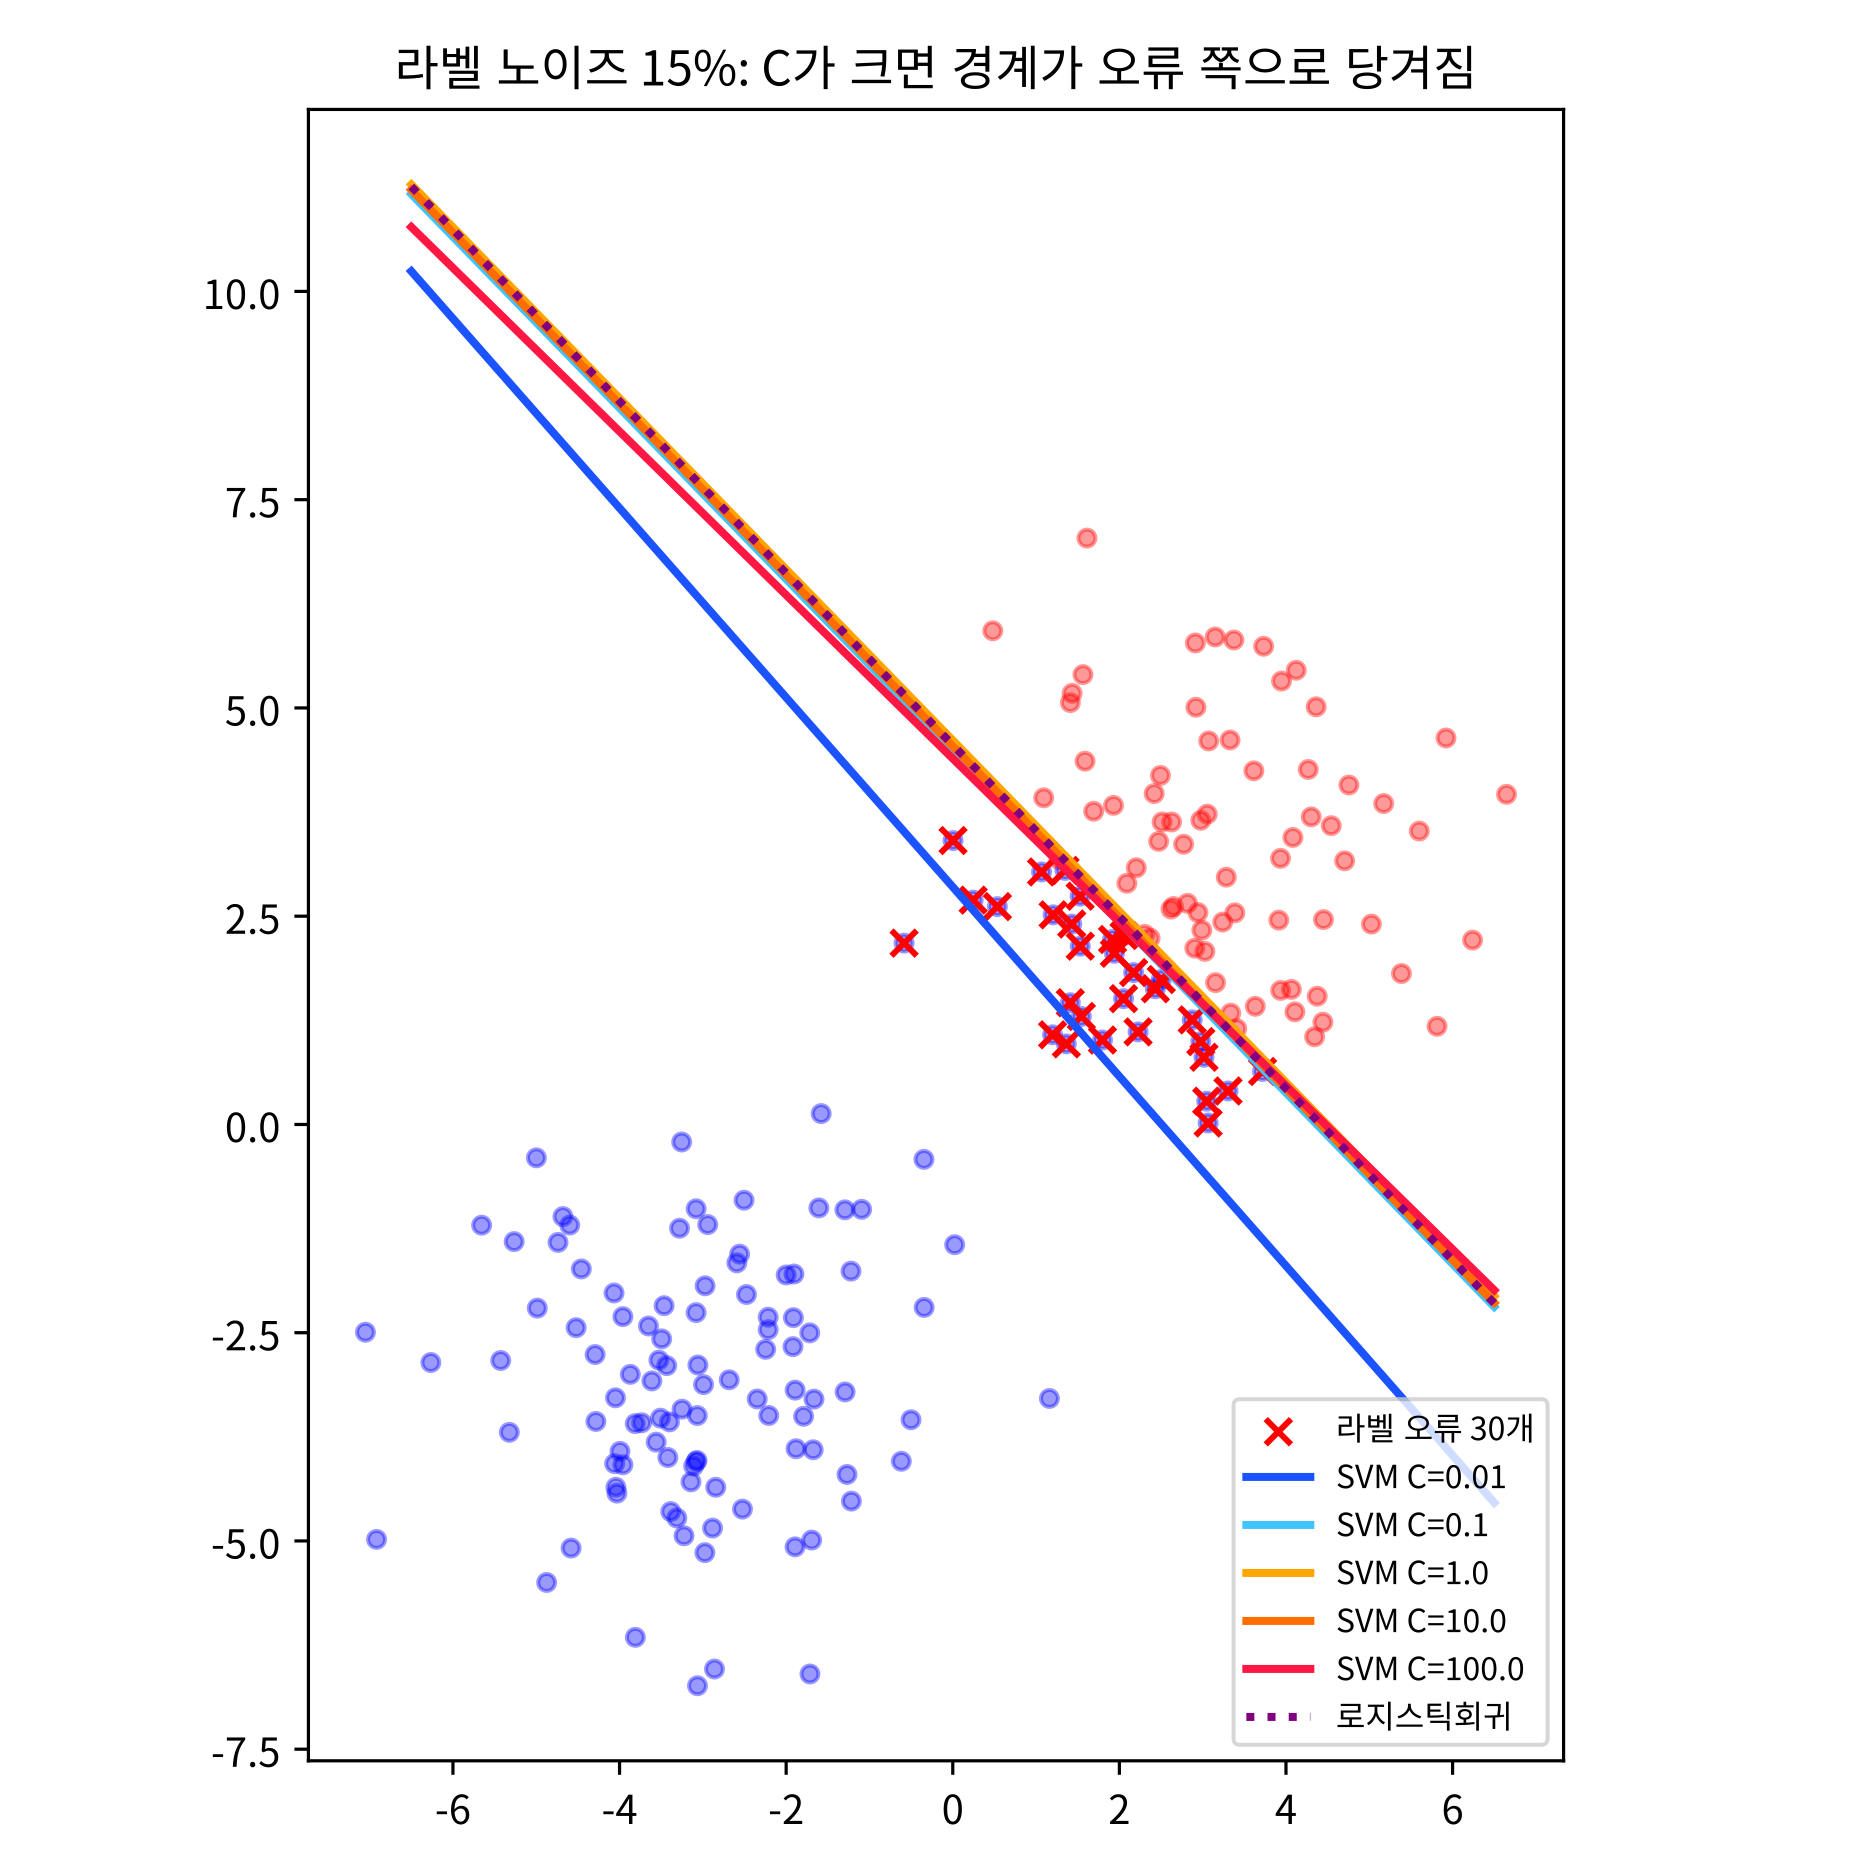
\includegraphics[width=\linewidth]{ch05_2_margin_boundary.png}
    \end{column}
    \begin{column}{0.44\textwidth}
      \small
      \begin{itemize}
        \item $C=0.01$(청색)의 경계가 라벨 오류(빨간 $\times$)
          \textbf{가장 멀리} 떨어져 있음.
        \item $C=100$(적색)과 로지스틱회귀(보라)가 오류 쪽으로
          \textbf{가장 가깝게} 밀려 있음.
        \item 로지스틱회귀 $\approx$ $C\approx1$의 SVM과 거의
          일치 — 교차 엔트로피가 힌지 손실과 ``거의 같은''
          모양이라 라벨 오류 반응이 유사.
      \end{itemize}
    \end{column}
  \end{columns}
\end{frame}

\begin{frame}{힌지 손실 vs 교차 엔트로피: ``기여가 사라지는'' 차이}
  $y=+1$인 점이 기능적 마진 $f$일 때, $w$ 그래디언트에 기여하는
  계수($y\,x$의 크기를 1로):
  \small
  \begin{tabular}{@{}ccc@{}}
    \toprule
    $f$ & 힌지 기여 & 교차엔트로피 기여 \\
    \midrule
    $-2.0$ & 3.0000 & 0.8808 \\
    $-1.0$ & 2.0000 & 0.7311 \\
    $-0.5$ & 1.5000 & 0.6225 \\
    $0.0$  & 1.0000 & 0.5000 \\
    $0.5$  & 0.5000 & 0.3775 \\
    $1.0$  & \textbf{0.0000} & 0.2689 \\
    $2.0$  & \textbf{0.0000} & 0.1192 \\
    $3.0$  & \textbf{0.0000} & 0.0474 \\
    \bottomrule
  \end{tabular}
  \normalsize\vskip0.4em
  \begin{columns}[T]
    \begin{column}{0.5\textwidth}
      \kb{힌지}
      \begin{itemize}
        \item $f\ge1$에서 \textbf{정확히 0} — 그 점을 아예 무시
        \item ``서포트 벡터만 경계를 결정''
      \end{itemize}
    \end{column}
    \begin{column}{0.5\textwidth}
      \kb{교차 엔트로피}
      \begin{itemize}
        \item 0으로 \textbf{수렴만} ( $f=3$에서도 0.047)
        \item ``모든 점이 손실에 계속 기여''
      \end{itemize}
    \end{column}
  \end{columns}
  \vskip0.4em
  실무적 함의: 이상치가 많으면 로지스틱회귀는 이상치가 아무리
  멀어도 (아주 작은 기울기로라도) 경계에 영향; SVM은 이상치가
  서포트 벡터가 안 되는 한(마진 바깥) \textbf{완전히 무시} —
  ``이상치 견고성''에서 \textbf{서로 다른 트레이드오프}.
\end{frame}

\begin{frame}[fragile]{실습: 힌지 손실 경사하강법 구현}
  \begin{lstlisting}
def hinge_loss_gradient_descent(X, y, C, alpha, epochs):
    # y[i]는 -1 또는 +1
    m, n = len(X), len(X[0])
    w, b = [0.0] * n, 0.0
    for _ in range(epochs):
        grad_w, grad_b = [0.0] * n, 0.0
        for i in range(m):
            margin = y[i] * (sum(w[j] * X[i][j] for j in range(n)) + b)
            if margin < 1:  # 마진을 위반한 점만 그래디언트에 기여
                for j in range(n):
                    grad_w[j] += -y[i] * X[i][j]
                grad_b += -y[i]
        for j in range(n):
            grad_w[j] = w[j] + C * grad_w[j] / m  # ||w||^2 항 + 힌지 항
        grad_b = C * grad_b / m
        for j in range(n):
            w[j] -= alpha * grad_w[j]
        b -= alpha * grad_b
    return w, b
\end{lstlisting}
\end{frame}

\begin{frame}{이 코드의 핵심 줄: \texttt{if margin < 1}}
  \begin{itemize}
    \item \texttt{if margin < 1} — 마진을 \textbf{만족한} 점
      ($f\ge1$)은 \texttt{grad\_w}, \texttt{grad\_b}에 \textbf{아무것도}
      더하지 않는다(힌지 손실의 비활성화 성질).
    \item $C \times \text{grad}$: $\frac12\|w\|^2$ 항(그래디언트 $w$)과
      힌지 항을 병합. $C$가 이 곱셈에 들어가므로
      \textbf{$C$가 클수록 힌지 위반에 대한 그래디언트가 상대적으로
      커진다} — ``이상치를 더 강하게 싫어한다''는 것을 옵티마이저가
      숫자로 느낌.
  \end{itemize}
  \vskip0.5em
  \begin{itemize}
    \item 5.1절 대칭 데이터에 적용하면 $w\approx(0.17,0.17)$, $b=0$ —
      정확해 $(1/6,1/6)$ 근처에서 힌지 손실의 ``꺾임'' 때문에
      약간 진동.
    \item 이상치가 들어간 데이터에 적용하면 $C$에 따라 $w, b$가
      달라지는 것을 직접 확인할 수 있다.
  \end{itemize}
\end{frame}

\begin{frame}{자주 하는 실수: $C$를 ``느낌''으로 고정하기}
  \begin{itemize}
    \item $C$를 한 번 정하면 그 값이 이상치를 얼마나 용인할지를
      사실상 \textbf{결정}해버린다.
    \item 흔한 실수: $C=1.0$(scikit-learn의 기본값) 같은 값을
      \textbf{별다른 검증 없이} 그대로 쓰는 것.
    \item 데이터에 라벨링 오류/이상치가 많이 섞여 있으면
      $C$가 너무 커서 소수 이상치에 과도하게 맞추려다
      \textbf{전체 경계가 왜곡}된다.
    \item 반대로 데이터가 매우 깨끗한데 $C$를 너무 작게 잡으면
      굳이 필요 없는 여유(마진)를 과하게 허용해
      \textbf{분류 성능을 낭비}.
  \end{itemize}
  \vskip0.5em
  \begin{block}{$C$는 검증셋으로 튜닝하는 하이퍼파라미터}
    2장의 학습률, 4장의 $k$와 마찬가지로 \textbf{검증셋 성능으로
    튜닝}해야 한다 — \texttt{sklearn.model\_selection.GridSearchCV}로
    여러 $C$ 값(로그 스케일로 0.01, 0.1, 1, 10, 100)을
    검증셋 정확도로 비교하는 것이 표준.
  \end{block}
\end{frame}

\begin{frame}{역사: ``허용하는 마진''의 아이디어}
  \begin{itemize}
    \item 소프트 마진의 수학적 형식(여유 변수 + $C$ 트레이드오프)은
      Cortès \& Vapnik (1995) \textit{``Support-Vector Networks''}에서
      완성.
    \item ``순수 기하학'' 이미지보다 \textbf{조금 더 실용적} —
      하드 마진은 ``완벽한 분리''를 가정하지만 실전 데이터는 항상
      노이즈가 있으므로, \textbf{실용적으로 쓸 수 있는 SVM은
      사실상 소프트 마진 버전뿐}.
    \item scikit-learn의 \texttt{SVC}는 하드 마진을 \textbf{지원하지
      않음}(항상 $C$를 받음) — ``하드 마진''이 필요한 상황도
      $C = 10^9$ 정도의 큰 값으로 대체.
  \end{itemize}
  \vskip0.5em
  \begin{block}{$1/C$가 정규화 세기와 정확히 대응}
    목적함수를 데이터 수 $m$ 기준으로 쓰면
    \[
    \frac{1}{2m}\|w\|^2 + \lambda\sum \xi
    \qquad (\lambda = 1/(mC))
    \]
    6장의 L2 정규화 $\frac{\lambda}{2}\|w\|^2 + \text{손실}$과
    \textbf{구조적으로 동일한 형태}.
    \vskip0.3em
    ``SVM의 $C$ 튜닝''과 ``로지스틱회귀의 정규화 세기 $\lambda$ 튜닝''은
    \textbf{같은 종류}의 하이퍼파라미터 튜닝 — $C$가 작을수록
    모델이 더 단순(편향$\uparrow$ 분산$\downarrow$).
  \end{block}
\end{frame}

\begin{frame}{이 절의 핵심 세 가지}
  \begin{enumerate}
    \item \kb{소프트 마진 = ``제약 풀기 + 위반 페널티'':}
      $y(w^\top x+b)\ge1$을 $y(w^\top x+b)\ge 1-\xi^{(i)}$로 풀어놓고
      $C\sum\xi$를 목적함수에 더함. $C$가 이 트레이드오프의 손잡이.
    \item \kb{$C$는 항상 검증셋으로 튜닝}:
      $C\to\infty$는 하드 마진(이상치에 취약), $C\to0$은 아무것도
      분류하지 않는 모델. \textbf{라벨 노이즈가 많을수록 작은 $C$}.
    \item \kb{힌지 손실의 ``비활성화'' 성질}이 서포트 벡터 개념을
      가능하게 함 — 마진 바깥의 점은 경계에 아무 영향을 주지 않는다.
  \end{enumerate}
  \vskip0.6em
  \begin{block}{5.3절(커널 트릭)으로 넘어가기 전, 연결고리}
    소프트 마진 목적함수 $\frac12\|w\|^2 + C\sum\xi$에서 $w^\top x$가
    \textbf{내적} 형태로만 등장한다. 커널 트릭은 이 $w^\top x$를
    $K(x,x')$로 대체하는 것 — \textbf{소프트 마진 목적함수는
    그대로 두고, 내적만 커널로 바꾼다}.
  \end{block}
\end{frame}

\begin{frame}{자주 묻는 질문 (1/2)}
  \textbf{Q. $C$가 무한대에 가까워지면?}
  \begin{itemize}
    \item $C\to\infty$: 아주 작은 위반($\xi^{(i)}>0$)에도 목적함수가
      \textbf{폭발} $\Rightarrow$ 사실상 위반을 전혀 허용하지 않는
      5.1절 \textbf{하드 마진}과 같아짐.
    \item $C\to0$: 위반 페널티가 사라져 마진을 최대로 넓히는 것
      ($w=0$)만 남음 — \textbf{아무것도 분류하지 않는} 모델.
    \item 그래서 $C$는 항상 이 두 극단 사이의 \textbf{적당한 값}을
      찾는 문제.
  \end{itemize}
  \vskip0.5em
  \textbf{Q. 힌지 손실 vs 교차 엔트로피의 차이?}
  \begin{itemize}
    \item 둘 다 ``마진(확률)이 부족할수록 손실 커진다''.
    \item 힌지는 마진이 \textbf{충분하면}($\ge1$) 손실이 \textbf{정확히
      0}이 되어 그 점에 더 이상 신경 쓰지 않음.
    \item 교차 엔트로피는 아무리 확신 있게 맞혀도 손실이 정확히 0이
      안 되고 계속 아주 조금씩 줄어듦.
  \end{itemize}
\end{frame}

\begin{frame}{자주 묻는 질문 (2/2)}
  \textbf{Q. 서포트 벡터의 개수가 $C$에 따라 변하나?}
  \begin{itemize}
    \item C 스윕 표에서: $C=0.01$ $\to$ 14개, $C=0.1$ $\to$ 5개,
      $C\ge1$ $\to$ 2개.
    \item \textbf{$C$가 작을수록 SV가 많아짐} — 이상치를 무시하고
      마진을 넓히려면 더 많은 점이 마진 경계에 달라붙어야 하므로.
    \item SV 개수 = SVM의 \textbf{효과적 모델 크기}(예측 시
      비교할 점의 수) — $C$ 튜닝의 부수적 효과로 ``모델의 간결함''도
      함께 조절.
  \end{itemize}
  \vskip0.5em
  \textbf{Q. 이상치가 \textbf{많이} 있으면 $C$ 튜닝으로 해결되지 않나요?}
  \begin{itemize}
    \item 이상치가 \textbf{데이터의 상당 부분}(예: 30\% 이상)이면
      어느 쪽을 택해도 일반화 성능이 떨어짐 — 작은 $C$는 진짜
      신호도 함께 무시, 큰 $C$는 노이즈에 과적합.
    \item 이런 때는 \textbf{모델이 아니라 데이터 자체}의 문제를 먼저:
      라벨링 품질 점검, 이상치 탐지(4장 kNN, 8장 앙상블),
      \textbf{주변부 잘라내기}(클러스터 밖에 고립된 의심점 전처리
      제거).
    \item $C$는 ``몇 \% 수준의 노이즈''를 조절하는 손잡이지,
      ``데이터의 절반이 틀린'' 문제를 해결하는 \textbf{마법이
      아니다}.
  \end{itemize}
\end{frame}

% =====================================================================
\section{5.3 커널 트릭: 선형분리가 안 되는 데이터}

\begin{frame}{도입: 5.1$\sim$5.2절이 놓친 마지막 벽}
  \begin{itemize}
    \item 5.1 하드 마진: 선형분리 가능을 \textbf{전제}
    \item 5.2 소프트 마진: 그 전제는 포기했으나, \textbf{결정 경계가
      직선}이라는 전제는 여전히 유지
    \item 이번 절의 데이터: 노이즈가 \textbf{없어도} 직선으로는
      \textbf{원리적으로} 못 나뉨
  \end{itemize}
  \vskip0.5em
  \begin{columns}[T]
    \begin{column}{0.5\textwidth}
      \kb{XOR}
      \begin{itemize}
        \item 네 클러스터($\pm1$ 근처)에서 1·3사분면 = A,
          2·4사분면 = B.
        \item 직선은 ``한쪽 끝과 반대쪽 끝''을 가를 뿐,
          \textbf{대각선}은 가를 수 없다.
      \end{itemize}
    \end{column}
    \begin{column}{0.5\textwidth}
      \kb{동심원}
      \begin{itemize}
        \item 안쪽 원과 바깥쪽 원의 두 클래스.
        \item 직선이 아니라 \textbf{원}으로만 나뉨.
      \end{itemize}
    \end{column}
  \end{columns}
  \vskip0.5em
  이 두 패턴은 실전에서 ``선형 특징으로 설명되지 않는 비선형
  관계''의 축소판.
  \vskip0.4em
  \begin{center}
  \kq{경계를 휘게 하면서도 5.1절의 모든 재산(마진 최대화,\\
      서포트 벡터, $2/\|w\|$ 공식)을 유지할 수 있을까?}
  \end{center}
\end{frame}

\begin{frame}{고차원으로 옮기면 보이는 것: 동심원}
  $x=(x_1,x_2)$ 를 $\phi(x) = (x_1, x_2, x_1^2+x_2^2)$ 로 올리면:
  \begin{itemize}
    \item $x_1^2+x_2^2$ = \textbf{원점으로부터의 거리 제곱}이므로
    \item 안쪽 원환체(반경 $\sim0.4$)의 모든 점 $\to$
      한 고도 $z \approx 0.4^2 = 0.16$ 에,
    \item 바깥쪽 원환체(반경 $\sim1.0$)의 모든 점 $\to$
      다른 고도 $z \approx 1.0^2 = 1.0$ 에 붙는다.
    \item 2차원에서 원 둘레를 따라 ``동일한'' 점이던 것이,
      세 번째 축 $z$를 추가하는 순간 두 개의 \textbf{수평 고도}로
      벌어진다 — \textbf{수평 평면} $z=0.5$ 하나로 완벽히 분리.
    \item 3차원의 평면은 원래 공간으로 투영하면 \textbf{원}이 되므로,
      ``3차원의 평평한 경계'' $\equiv$ ``2차원의 원형 경계''.
  \end{itemize}
  \vskip0.4em
  {\footnotesize \texttt{make\_circles}에선 바깥쪽 원환체=클래스 0,
  안쪽=클래스 1 — 라벨 번호는 임의, ``두 고도로 벌어진다''는
  구조는 동일.}
\end{frame}

\begin{frame}{그림으로 읽기: 고도로 벌리면 평면이 자른다}
  \begin{columns}[T]
    \begin{column}{0.52\textwidth}
      \centering
      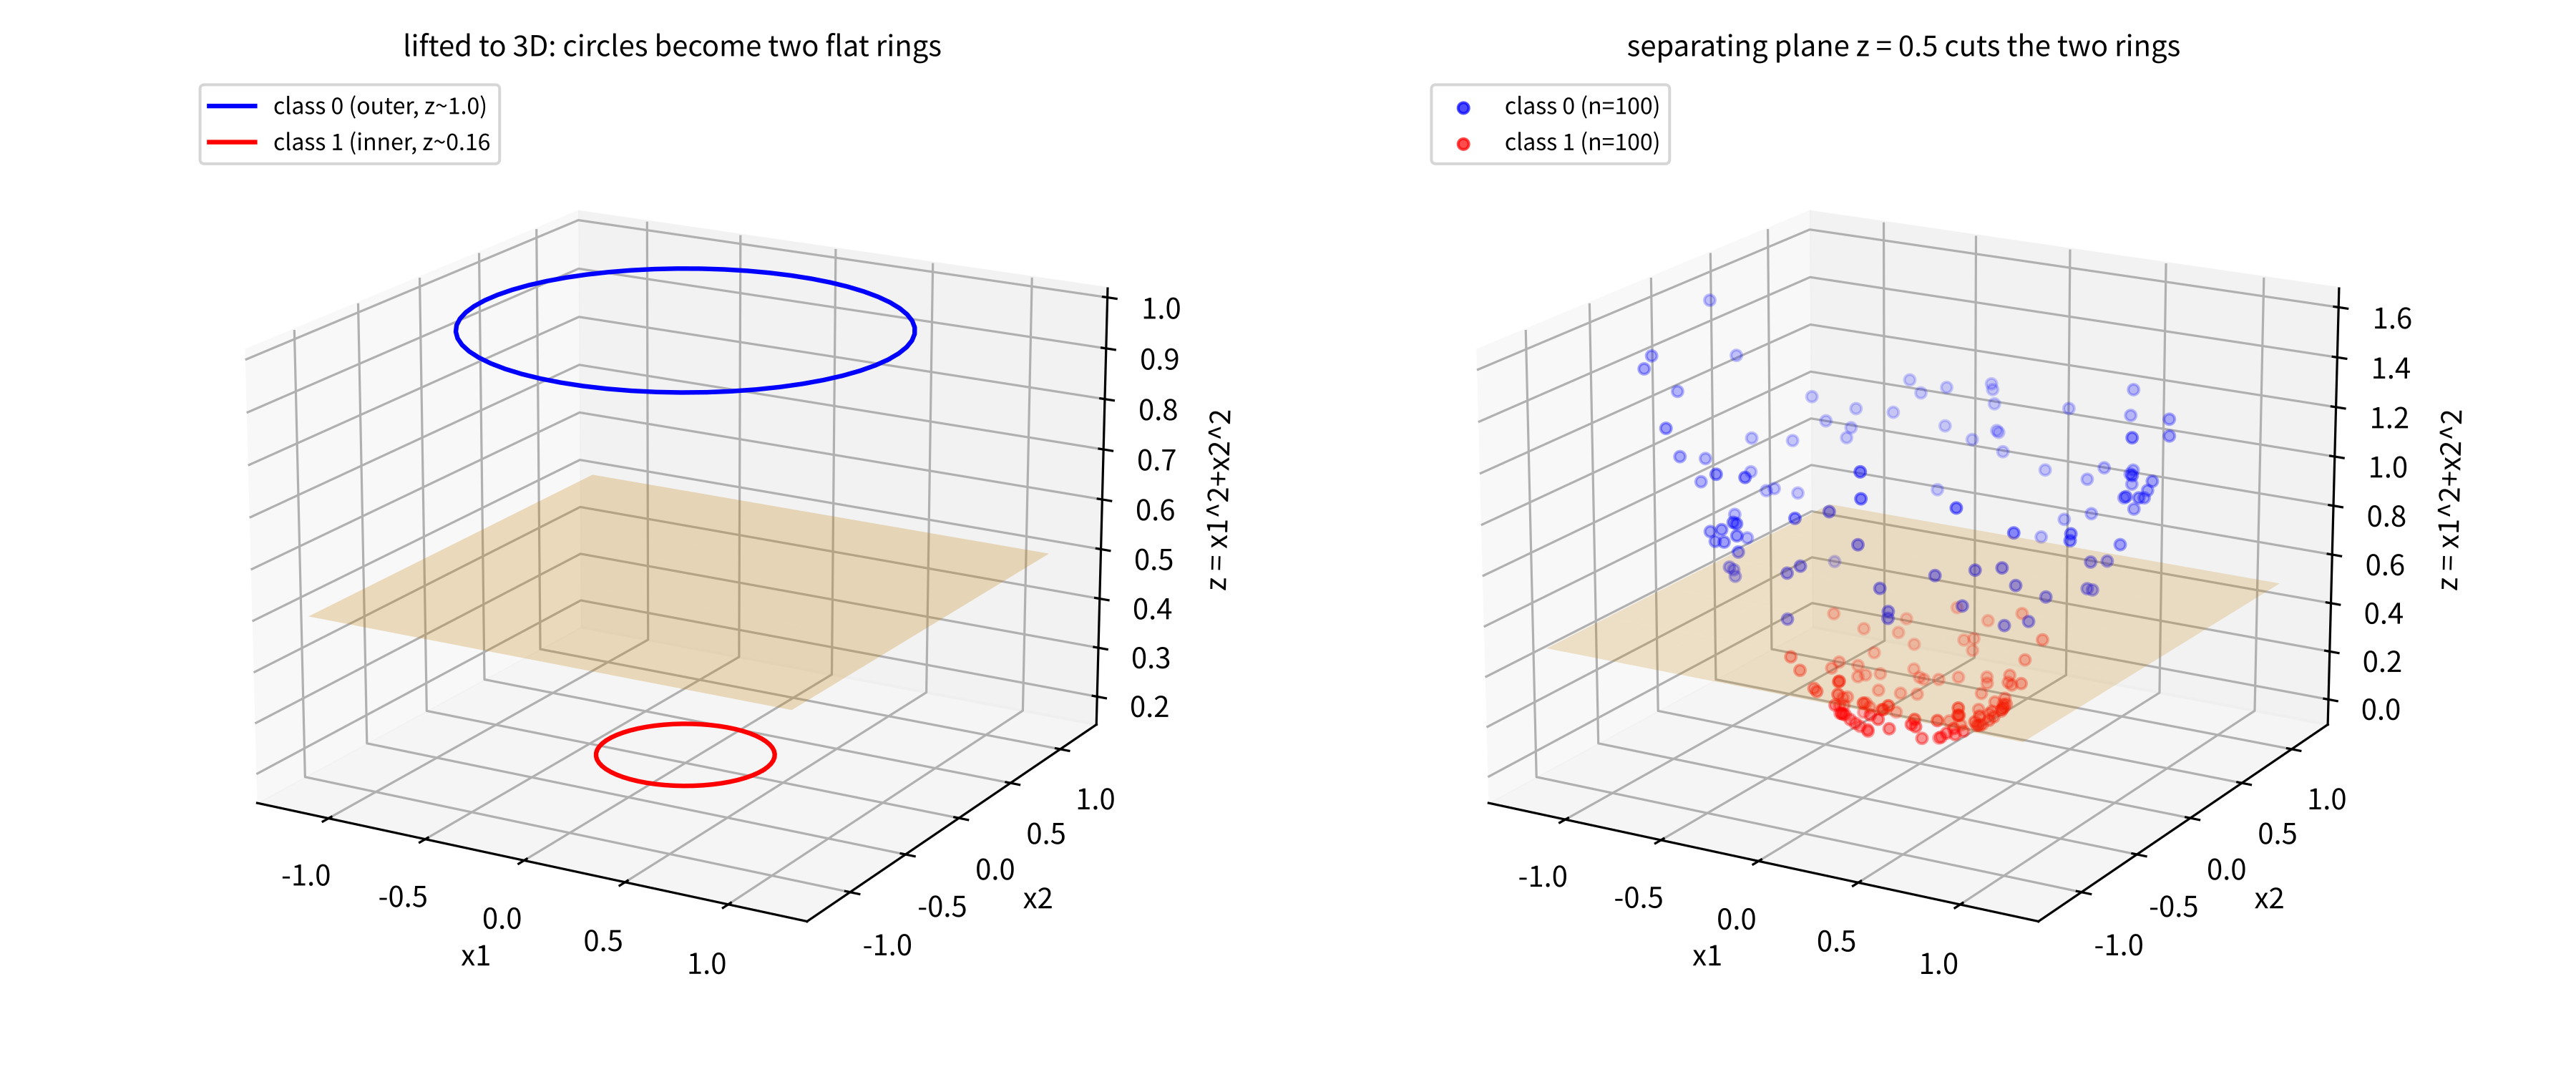
\includegraphics[width=\linewidth]{ch05_3_circles_3d_lift.png}
    \end{column}
    \begin{column}{0.44\textwidth}
      \small
      \begin{itemize}
        \item 좌: 동심원 데이터를 $z = x_1^2+x_2^2$ 축 위로
          올려보냄.
        \item 우: 두 원환체가 서로 다른 두 고도에 놓여
          \textbf{수평 평면 $z=0.5$ 하나로 잘림}.
        \item 3차원의 \textbf{평평한} 평면이 2차원으로 투영되면
          \textbf{원형} 경계가 됨.
      \end{itemize}
      \vskip0.5em
      \begin{block}{일반 원리}
        원래 공간에서 ``\textbf{곡면으로만} 나뉘는'' 관계는, 그
        곡면의 \textbf{고도를 새 특징으로} 추가하면 ``\textbf{평면으로
        나뉘는}'' 관계가 된다.
      \end{block}
      {\footnotesize XOR도 같은 식: $(x_1,x_2,x_1x_2)$ 로 올리면
      사분면 교차가 $x_3$ 축의 수평 평면 분리 문제.}
    \end{column}
  \end{columns}
\end{frame}

\begin{frame}{차원 문제, 그리고 커널 트릭 한 문장}
  \begin{itemize}
    \item $\phi(x)$ 를 명시적으로 계산하면 \textbf{차원이 감당
      못 하게} 커진다:
      다항식 특징을 도수 $d$까지 추가하면 $\binom{n+d}{d}$ 개,
      RBF는 \textbf{무한} 개.
    \item \kb{커널 트릭}(kernel trick, Cortès \& Vapnik 1995)은 이걸
      \textbf{피해간다}:
    \begin{itemize}
      \item SVM의 최적화 문제를 \textbf{라그랑주 쌍대}로 다시 쓰면,
        데이터가 항상 $\phi(x^{(i)})\cdot\phi(x^{(j)})$
        (\textbf{내적}) 형태로만 등장함을 알 수 있다.
      \item 그러면 $\phi$ 를 직접 계산하지 않고, 이 내적값을
        \textbf{곧바로} 계산해주는 \kb{커널 함수}
        $K(x,x') = \phi(x)\cdot\phi(x')$ 만 있으면 충분.
    \end{itemize}
  \end{itemize}
  \vskip0.6em
  \begin{block}{이게 전부다}
    커널 트릭은 ``새로운 모델''이 아니라, \textbf{같은 모델의
    계산 방식을 고차원 내적으로만 다시 쓴 것}.
  \end{block}
\end{frame}

\begin{frame}{쌍대 문제: 내적이 드러나는 자리}
  5.1$\sim$5.2에선 primal $J(w,b)=\frac12\|w\|^2 + C\sum\xi^{(i)}$
  를 직접 풀었다. \textbf{라그랑주 쌍대}로 다시 쓰면
  (라그랑주 함수 구성, $w,b$ 최소화, KKT 조건까지의 완전한 유도 —
  이 책 범위 밖, ``쌍대가 어떻게 생겼는지''만):
  \[
  \text{최대화}\ \sum_i \alpha^{(i)}
  - \frac{1}{2}\sum_{i,j}\alpha^{(i)}\alpha^{(j)}y^{(i)}y^{(j)}
  \,\phi(x^{(i)})\cdot\phi(x^{(j)})
  \qquad \text{s.t.}\ \alpha^{(i)} \ge 0,\ \sum_i \alpha^{(i)} y^{(i)}=0
  \]
  \vskip0.3em
  \begin{itemize}
    \item $\phi$ 는 \textbf{단 한 곳} — 내적
      $\phi(x^{(i)})\cdot\phi(x^{(j)})$ — 에서만 나온다.
      이 내적값을 $K(x^{(i)},x^{(j)})$ 라는 \textbf{별개의 함수}로
      교체해도 \textbf{수학이 깨지지 않음}. $\phi$ 가 어떤 공간으로
      가는지도, 차원이 몇인지도 \textbf{알 필요 없음}.
  \end{itemize}
  \vskip0.3em
  \begin{block}{왜 내적으로만 나오게 된 것일까}
    직관: $w$=경계의 \textbf{방향}, $\alpha^{(i)}$=각 점이 경계를
    \textbf{떠받치는 세기}. KKT에 의해 비-SV의 $\alpha$ 는 0 $\Rightarrow$
    $w = \sum_{i\in \text{SV}} \alpha^{(i)} y^{(i)} \phi(x^{(i)})$
    (서포트 벡터의 \textbf{선형 결합}).
    $w$ 가 SV들의 합으로 표현되는 순간 $w^\top\phi(x^{(j)})$ 는
    $\sum_i \alpha^{(i)}y^{(i)}\,\phi(x^{(i)})\cdot\phi(x^{(j)})$
    로 펼쳐져 — 데이터의 등장 방식이 \textbf{내적 쌍}으로
    \textbf{통일}. ``내적 쌍''만 계산할 수 있으면 $\phi$ 자체는
    \textbf{영원히 볼 필요 없음}.
  \end{block}
\end{frame}

\begin{frame}{손으로 한 번: 6개 점을 2$\times$2 커널 행렬로}
  5.1절의 6개 대칭 데이터로 쌍대 문제를 직접 풀어
  \textbf{같은 해}가 나오는지 확인:
  \begin{itemize}
    \item SV는 $(3,3){\to}+1$과 $(-3,-3){\to}-1$ 두 점뿐.
      KKT에 의해 나머지 4개의 $\alpha$ 는 0 —
      \textbf{살아남는 알파는 두 개} $(\alpha_1, \alpha_4)$ 뿐.
    \item 제약 $\sum_i \alpha^{(i)}y^{(i)}=0$ 은
      $\alpha_1(+1)+\alpha_4(-1)=0$ $\Rightarrow$
      $\alpha_1 = \alpha_4 = a$ 강제.
    \item 쌍대 목적함수는 \textbf{일변수 2차함수}로 감소:
      \[
      f(a) = 2a - \frac12 a^2 q,
      \qquad
      q = y_1^2 K_{11} + y_4^2 K_{44} + 2y_1y_4 K_{14} = 72
      \]
  \end{itemize}
\end{frame}

\begin{frame}{2$\times$2 커널 행렬과 꼭짓점}
  SV 두 점의 \textbf{2$\times$2 커널(내적) 행렬}:
  \[
  K =
  \begin{pmatrix} (3,3)\cdot(3,3) & (3,3)\cdot(-3,-3) \\
  (3,3)\cdot(-3,-3) & (-3,-3)\cdot(-3,-3) \end{pmatrix}
  =
  \begin{pmatrix} 18 & -18 \\ -18 & 18 \end{pmatrix}
  \]
  \begin{itemize}
    \item $q = 18 + 18 + 2(1)(-1)(-18) = 72$.
    \item $f(a)$ 는 $f'(a) = 2 - q\,a = 0$ 에서 꼭짓점:
      $a^* = 2/q = 1/36$.
    \item KKT로 $w$ 를 복원:
      \[
      w = \sum_i \alpha^{(i)}y^{(i)}x^{(i)}
      = \tfrac{1}{36}(+1)(3,3) + \tfrac{1}{36}(-1)(-3,-3)
      = \left(\tfrac16,\ \tfrac16\right)
      \]
  \end{itemize}
  \vskip0.4em
  \begin{block}{결과: 5.1절의 primal 손계산 해와 숫자 하나까지 일치}
    $b=0$ (대칭성). 실습 노트 3부에서 이 계산을 코드로 돌려
    6개 제약의 기능적 마진 $[1,\ 1.1667,\ 1.1667,\ 1,\ 1.1667,\
    1.1667]$(두 SV만 정확히 $=1$)과 기하적 마진
    $2/\|w\|=8.485$까지 \textbf{primal과 동일}함을 확인.
    \vskip0.3em
    \kb{primal과 dual이 같은 해를 주는 것}(강렬한 쌍대성)은 SVM이
    \textbf{볼록 최적화} 문제이기 때문에 성립 — 이 절의 커널
    트릭 이야기 \textbf{자체}가 이 성질에 의존.
    \vskip0.3em
    우리가 계산한 것은 \textbf{2$\times$2 내적 행렬}뿐 — primal에선
    $w=(1/6,1/6)$ 을 직접 들고 다녔지만, 쌍대에선 $w$ 를 알
    \textbf{필요 없이} \textbf{커널값(내적)으로만} 복원. 이
    구조가 RBF처럼 $\phi$ 가 무한차원인 경우에도 그대로 작동.
  \end{block}
\end{frame}

\begin{frame}{커널 함수: 내적을 우회한다}
  가장 널리 쓰이는 커널:
  \begin{columns}[T]
    \begin{column}{0.5\textwidth}
      \kb{다항 커널}(polynomial)
      \[
      K(x,x') = (x\cdot x' + c)^d
      \]
      ``도수 $d$ 이하의 \textbf{모든 단항식}''을 내포.
      $(x\cdot x'+1)^d$ 를 전개하면 도수 $d$ 이하의 모든
      단항식 $x_1^{a_1}x_2^{a_2}\cdots$ ($a_1+a_2+\cdots\le d$)
      이 (일정한 계수로) 전부 섞여 나온다.
    \end{column}
    \begin{column}{0.5\textwidth}
      \kb{RBF(가우시안) 커널}
      \[
      K(x,x') = \exp\Bigl(-\frac{\|x-x'\|^2}{2\sigma^2}\Bigr)
      \]
      두 점이 가까울수록 1에, 멀수록 0에 가까운 \textbf{유사도}
      함수. \textbf{무한 차원}의 $\phi$ 에 대응한다는 것이
      알려져 있는데도, 커널 함수 자체는 \textbf{유클리드 거리
      하나로} 계산.
    \end{column}
  \end{columns}
  \vskip0.4em
  {\footnotesize $\exp(-\gamma\|x-x'\|^2)$ 로 정의하는 문헌도
  많다 — $\gamma = 1/(2\sigma^2)$ 로 대응. scikit-learn의
  \texttt{SVC}는 \texttt{gamma}를 받는다.}
\end{frame}

\begin{frame}{다항 커널이 ``도수 2''를 정확히 어떻게 담는가}
  \begin{itemize}
    \item $d=2$: $(x\cdot x' + 1)^2$ 를 전개하면
      \[
      (x_1x_1' + x_2x_2')^2 + 2(x_1x_1' + x_2x_2') + 1
      \]
      $\Rightarrow$ 도수 2 ($x_1^2, x_2^2, x_1x_2$), 도수 1
      ($x_1, x_2$), 도수 0 (상수) 단항식 \textbf{전부} 포함.
    \item 명시적으로
      \[
      \phi_2(x) = (x_1^2,\ x_2^2,\ \sqrt{2}\,x_1x_2,\
      \sqrt{2}\,x_1,\ \sqrt{2}\,x_2,\ 1)
      \]
      로 쓰면 $\phi_2(x)\cdot\phi_2(x')$ 이 정확히
      $(x\cdot x'+1)^2$ 와 같음 — ``도수 2 이하 모든 단항식
      공간에서의 내적''이라는 $\phi$ 의 실체가 \textbf{6차원
      벡터}로 드러남.
  \end{itemize}
  \vskip0.5em
  \begin{block}{XOR에는 \textbf{도수 2}가 정확히 필요하다}
    사분면 교차를 만드는 핵심 단항식이 $x_1x_2$(도수 2)이므로:
    \textbf{도수 1}(=선형)은 원점을 기준으로 교차하는 양 클래스를
    직선 하나로 못 나누어 50\% 근처에 머물고, \textbf{도수 2}는
    $x_1x_2$ 항을 포함해 거의 완벽.
    \vskip0.3em
    실습에서 $d=1$은 정확도 0.74, $d=2$는 1.00 —
    \textbf{커널의 ``도수'' 하나만 바꿨을 뿐}.
  \end{block}
\end{frame}

\begin{frame}[fragile]{RBF 커널: ``봉우리''의 유사도}
  $K(x,x') = e^{-\|x-x'\|^2/2\sigma^2}$ 는 두 점이 가까우면
  $\approx1$, 멀면 $\approx0$ 인 ``얼마나 닮았는가''를 재는 함수.
  \begin{lstlisting}
def rbf_kernel(x1, x2, sigma):
    sq_dist = sum((x1[i] - x2[i]) ** 2 for i in range(len(x1)))
    return math.exp(-sq_dist / (2 * sigma ** 2))
\end{lstlisting}
  \begin{columns}[T]
    \begin{column}{0.5\textwidth}
      \kb{$\sigma$ 작다}(좁은 봉우리)
      \begin{itemize}
        \item 아주 가까운 점만 ``비슷''
        \item $\gamma$ 큼 $\Rightarrow$ 경계 \textbf{구불}
        \item 과적합 위험
      \end{itemize}
    \end{column}
    \begin{column}{0.5\textwidth}
      \kb{$\sigma$ 크다}(넓은 봉우리)
      \begin{itemize}
        \item 멀리 있는 점도 ``비슷''
        \item $\gamma$ 작음 $\Rightarrow$ 경계 \textbf{단순}
        \item 과소적합 위험
      \end{itemize}
    \end{column}
  \end{columns}
  \vskip0.3em
  {\footnotesize 이 ``봉우리'' 관점이 중요한 이유: RBF 커널 SVM의
  \textbf{예측값}은 ``새 점이 각 서포트 벡터와 얼마나 비슷한가''
  (커널값)를 \textbf{가중 투표}하는 형태.}
\end{frame}

\begin{frame}{RBF의 무한차원 실체, 실효 차원, 머서 조건}
  ``RBF 커널은 무한차원의 $\phi$ 에 대응한다'' — 구체적으로:
  \begin{itemize}
    \item $\|x-x'\|^2 = \|x\|^2+\|x'\|^2 - 2x\cdot x'$ 로 넣고
      $e^{2\gamma\, x\cdot x'}$ 를 테일러 전개하면, $\phi(x)$ 는
      \textbf{모든 도수의 모든 단항식}에 가우시안 인자를 둔
      \textbf{무한}개의 성분 $\phi_\alpha(x)$ 를 가진다.
    \item \kb{실효 차원은 데이터 개수로 제한된다}: $m$개 데이터의
      커널(Gram) 행렬 $K_{ij}=K(x_i,x_j)$ 의 \textbf{랭크는 최대
      $m$} — $\phi$ 가 무한차원이어도 실제로 ``활용하는'' 특징
      차원은 \textbf{데이터 수를 넘지 않음}.
      (실습: 60개 4차원 RBF 커널 행렬이 rank 60임을 고유값으로 확인)
  \end{itemize}
  \vskip0.4em
  \begin{block}{머서(Mercer) 조건 — 유효 커널의 필요 조건}
    커널 함수가 유효하려면 커널 행렬이 \textbf{모든} 데이터에 대해
    \textbf{양의 준정부호}(모든 고유값 $\ge 0$)여야 한다.
    RBF: 60개 4차원($\gamma=0.5$)에서 최소 고유값
    $5.07\times10^{-3}>0$, 랭크 60 — 직접 확인.
    유한 절단만으로도 꽤 정확한 근사 — ``무한차원''은
    \textbf{개념적} 차원일 뿐 계산 비용이 무한하다는 뜻이 \textbf{아님}.
  \end{block}
\end{frame}

\begin{frame}[fragile]{실습: RBF 커널로 비선형 분류}
  \begin{lstlisting}
from sklearn.datasets import make_circles
from sklearn.svm import SVC
from sklearn.model_selection import train_test_split

X, y = make_circles(n_samples=200, noise=0.1, factor=0.4, random_state=0)
X_train, X_test, y_train, y_test = train_test_split(
    X, y, test_size=0.3, random_state=0)

linear_svm = SVC(kernel="linear").fit(X_train, y_train)
rbf_svm    = SVC(kernel="rbf", gamma=2.0).fit(X_train, y_train)

print("선형 커널 정확도:", round(linear_svm.score(X_test, y_test), 3))
print("RBF 커널 정확도: ", round(rbf_svm.score(X_test, y_test), 3))
\end{lstlisting}
  \vskip0.3em
  {\footnotesize \texttt{make\_circles}: 바깥쪽 원환체(클래스 0,
  반경 $\sim1.0$)와 안쪽 원환체(클래스 1, 반경 $\sim0.4$)가 동심원
  모양으로 얽혀 있어 \textbf{어떤 직선으로도 나눌 수 없음}.
  라벨 번호는 임의 배정에 불과 — 결과와 무관.}
\end{frame}

\begin{frame}{그림으로 읽기: 커널 하나만 바꿨을 뿐}
  \begin{columns}[T]
    \begin{column}{0.52\textwidth}
      \centering
      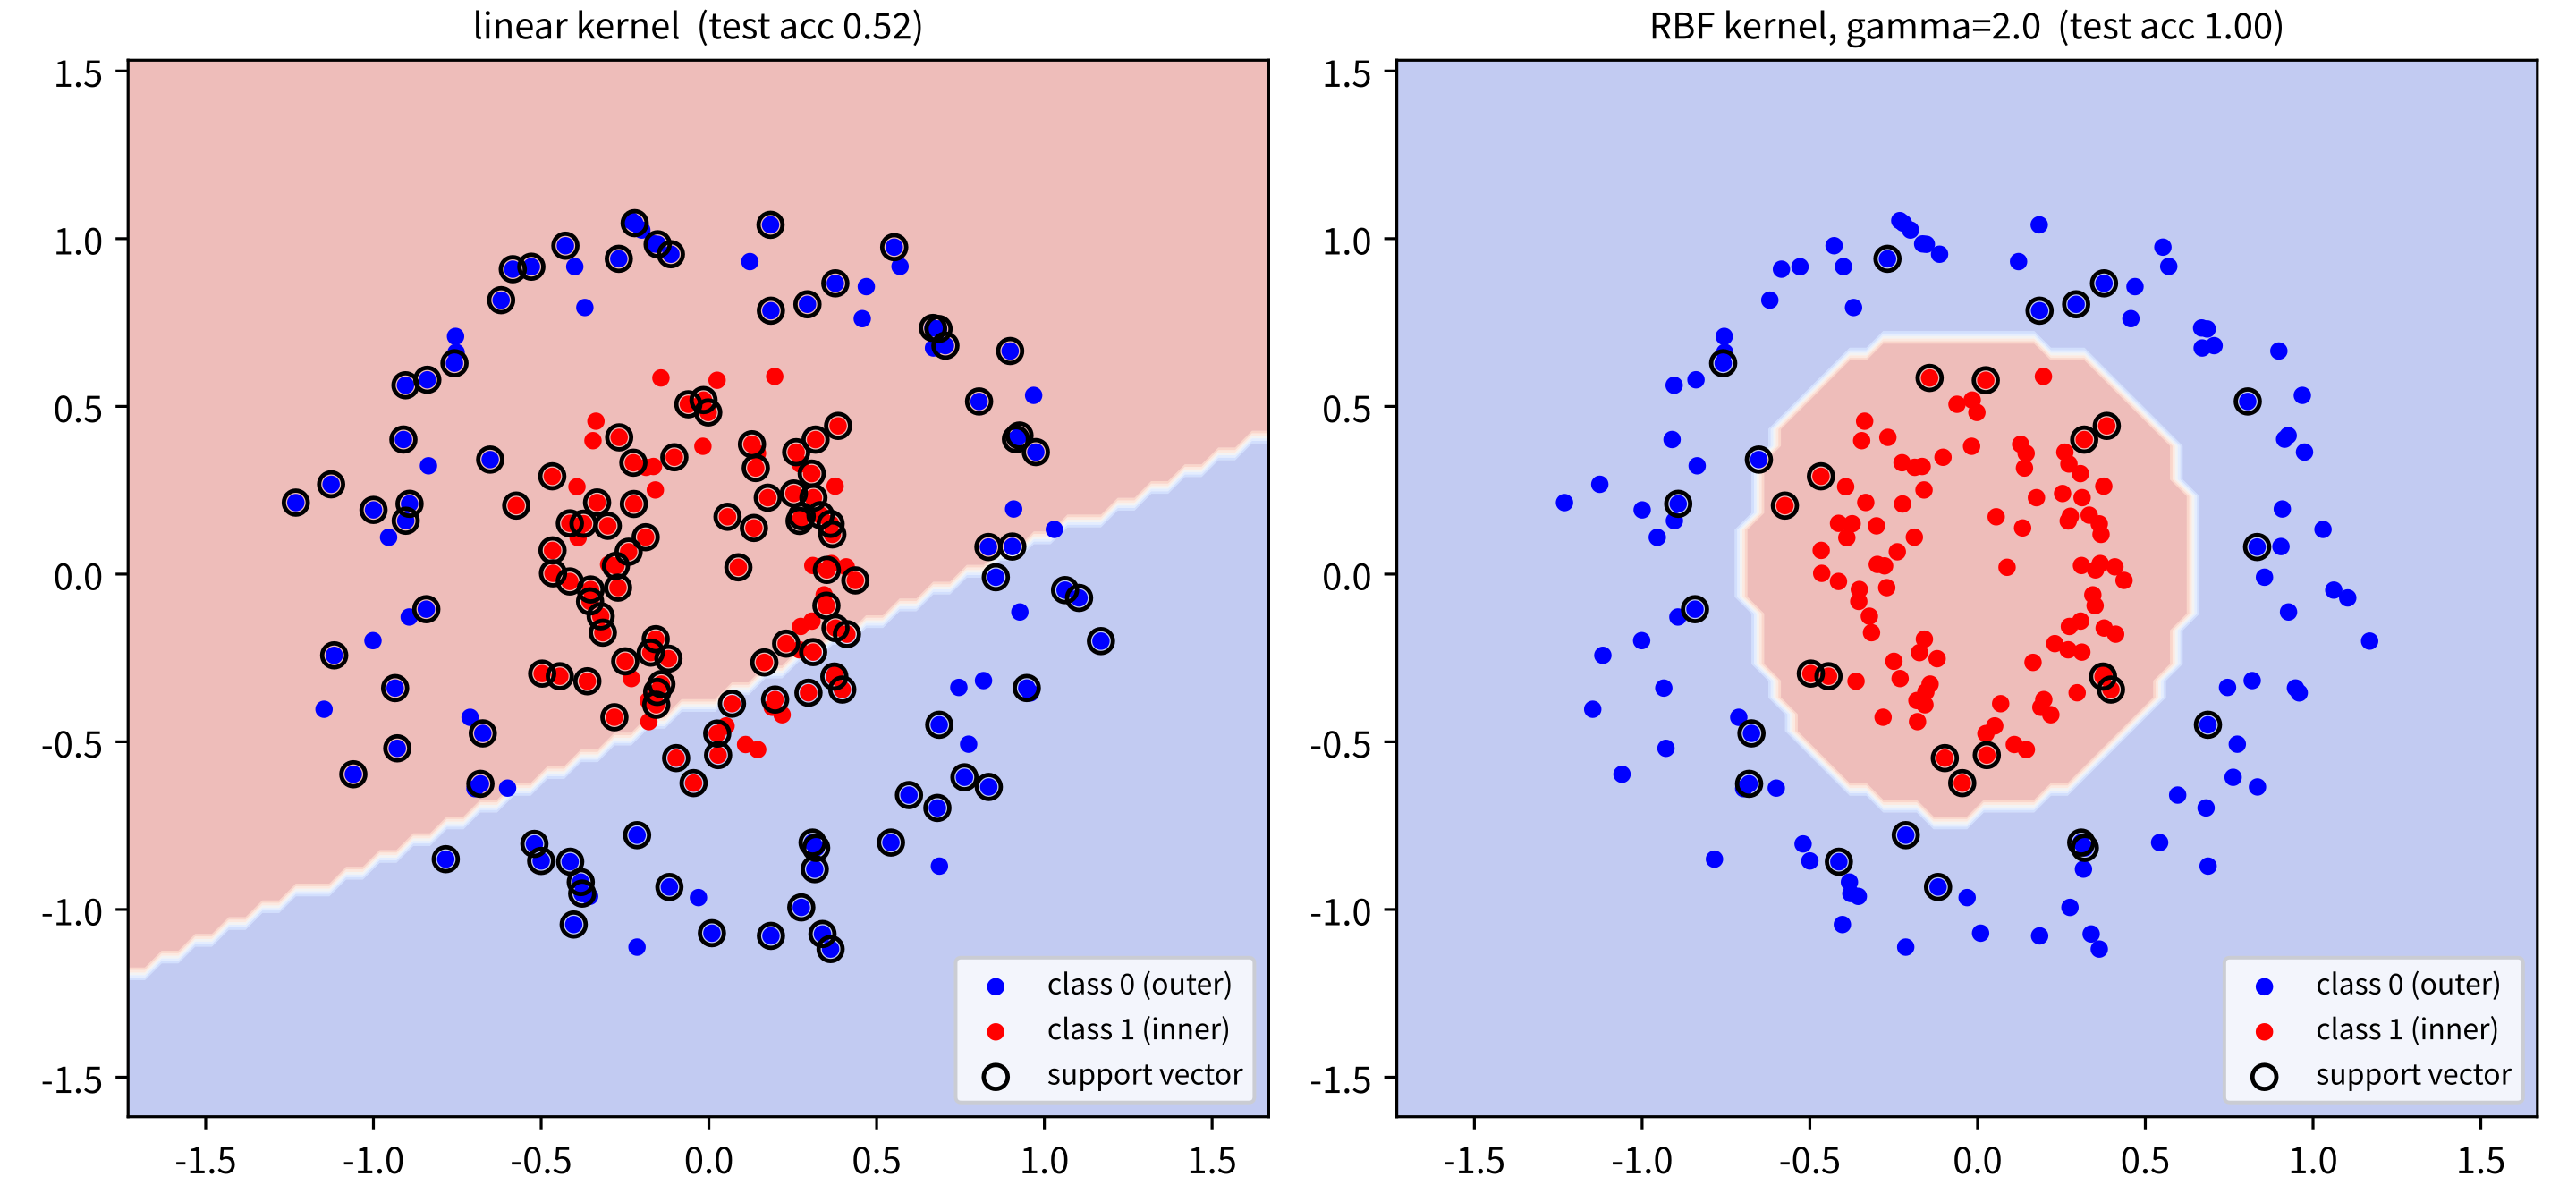
\includegraphics[width=\linewidth]{ch05_3_kernel_boundaries.png}
    \end{column}
    \begin{column}{0.44\textwidth}
      \small
      \begin{itemize}
        \item \kb{선형 커널}(좌): 동심원을 직선 하나로 어정쩡하게
          자를 뿐 — 정확도 \textbf{0.52}(동전 던지기 수준).
        \item \kb{RBF 커널}(우): \textbf{원형 결정 경계}로 안쪽·
          바깥쪽 원을 완벽히 분리 — 정확도 \textbf{1.00}.
      \end{itemize}
      \vskip0.4em
      \begin{block}{서포트 벡터 개수가 핵심}
        선형 커널: 학습 데이터 \textbf{137개}$(\approx68\%)$를
        SV로 끌고 옴.
        RBF 커널: \textbf{31개}만 SV로 쓰고 나머지 169개는
        마진 바깥에 둠.
        \vskip0.3em
        5.2절의 ``서포트 벡터가 경계를 떠받친다''는 원칙이
        \textbf{비선형 경계에도 그대로} 적용되는 직접적 증거.
      \end{block}
    \end{column}
  \end{columns}
\end{frame}

\begin{frame}[fragile]{실습: $\gamma$ 스윕 — 경계가 얼마나 구불거릴 수 있는가}
  \begin{lstlisting}
def plot_boundary(ax, clf, title, data=X, ydata=y):
    h = 0.05
    lims = [data[:,0].min()-0.5, data[:,0].max()+0.5,
            data[:,1].min()-0.5, data[:,1].max()+0.5]
    xx, yy = np.meshgrid(np.arange(lims[0], lims[1], h),
                         np.arange(lims[2], lims[3], h))
    Z = clf.predict(np.c_[xx.ravel(), yy.ravel()]).reshape(xx.shape)
    ax.contourf(xx, yy, Z, alpha=0.35, cmap="coolwarm")
    ax.scatter(data[ydata==0,0], data[ydata==0,1], c="blue", s=15,
               label="class 0 (outer)")
    ax.scatter(data[ydata==1,0], data[ydata==1,1], c="red",  s=15,
               label="class 1 (inner)")
    ax.scatter(X_train[clf.support_][:,0], X_train[clf.support_][:,1],
               s=45, facecolors="none", edgecolors="k", lw=1.2,
               label="support vector")
    ax.set_title(title, fontsize=10); ax.set_aspect("equal")
    ax.legend(loc="lower right", fontsize=8)

fig, axes = plt.subplots(2, 2, figsize=(10, 9))
for ax, g in zip(axes.ravel(), [0.05, 0.3, 1.0, 30.0]):
    clf = SVC(kernel="rbf", gamma=g, C=1.0).fit(X_train, y_train)
    print(f"gamma={g:5.2f} : train {clf.score(X_train,y_train):.3f}  "
          f"test {clf.score(X_test,y_test):.3f}  SV {len(clf.support_)}")
    plot_boundary(ax, clf, f"gamma = {g}   (test acc {clf.score(X_test,y_test):.2f})")
fig.suptitle("RBF gamma sweep on concentric circles", fontsize=12)
plt.show()
\end{lstlisting}
\end{frame}

\begin{frame}{$\gamma$ 스윕 결과: 4단계}
  \small
  \begin{tabular}{@{}cccc@{}}
    \toprule
    $\gamma$ & train acc & test acc & 서포트 벡터 수 \\
    \midrule
    0.05 & 0.514 & \textbf{0.467} & 136 \\
    0.30 & 0.993 & \textbf{1.000} & 74 \\
    1.00 & 1.000 & \textbf{1.000} & 34 \\
    30.00& 1.000 & \textbf{1.000} & 85 \\
    \bottomrule
  \end{tabular}
  \normalsize\vskip0.5em
  \begin{itemize}
    \item \kb{$\gamma=0.05$}: 경계가 \textbf{거의 직선}에 가깝게
      뭉뚱그려져 동심원을 아예 분리 못함(0.47 — 선형 커널보다도
      나쁨, \textbf{과소적합}).
    \item \kb{$\gamma=0.3$}: 원형 경계가 생기며 정확도가 1.0으로
      오름.
    \item \kb{$\gamma=30$}: 각 점마다 좁은 봉우리가 생겨 경계가
      학습 데이터 하나하나를 감싸는 형태로 \textbf{심하게
      구불거림}(SV 85개 증가).
  \end{itemize}
  \vskip0.3em
  이 동심원은 노이즈가 적어 큰 $\gamma$에서도 acc=1.00을 유지하지만
  (운 좋게 일반화되는 것이지), \textbf{실제 노이즈 있는 데이터}에선
  $\gamma=30$ 경계는 개별 노이즈 패턴까지 따라붙어 test가 급락 —
  4.1절 kNN의 작은 $k$, 5.2절의 큰 $C$와 \textbf{정확히 같은
  종류}의 과적합.
\end{frame}

\begin{frame}{그림으로 읽기: $\gamma$ 4단계 한눈에}
  \begin{columns}[T]
    \begin{column}{0.52\textwidth}
      \centering
      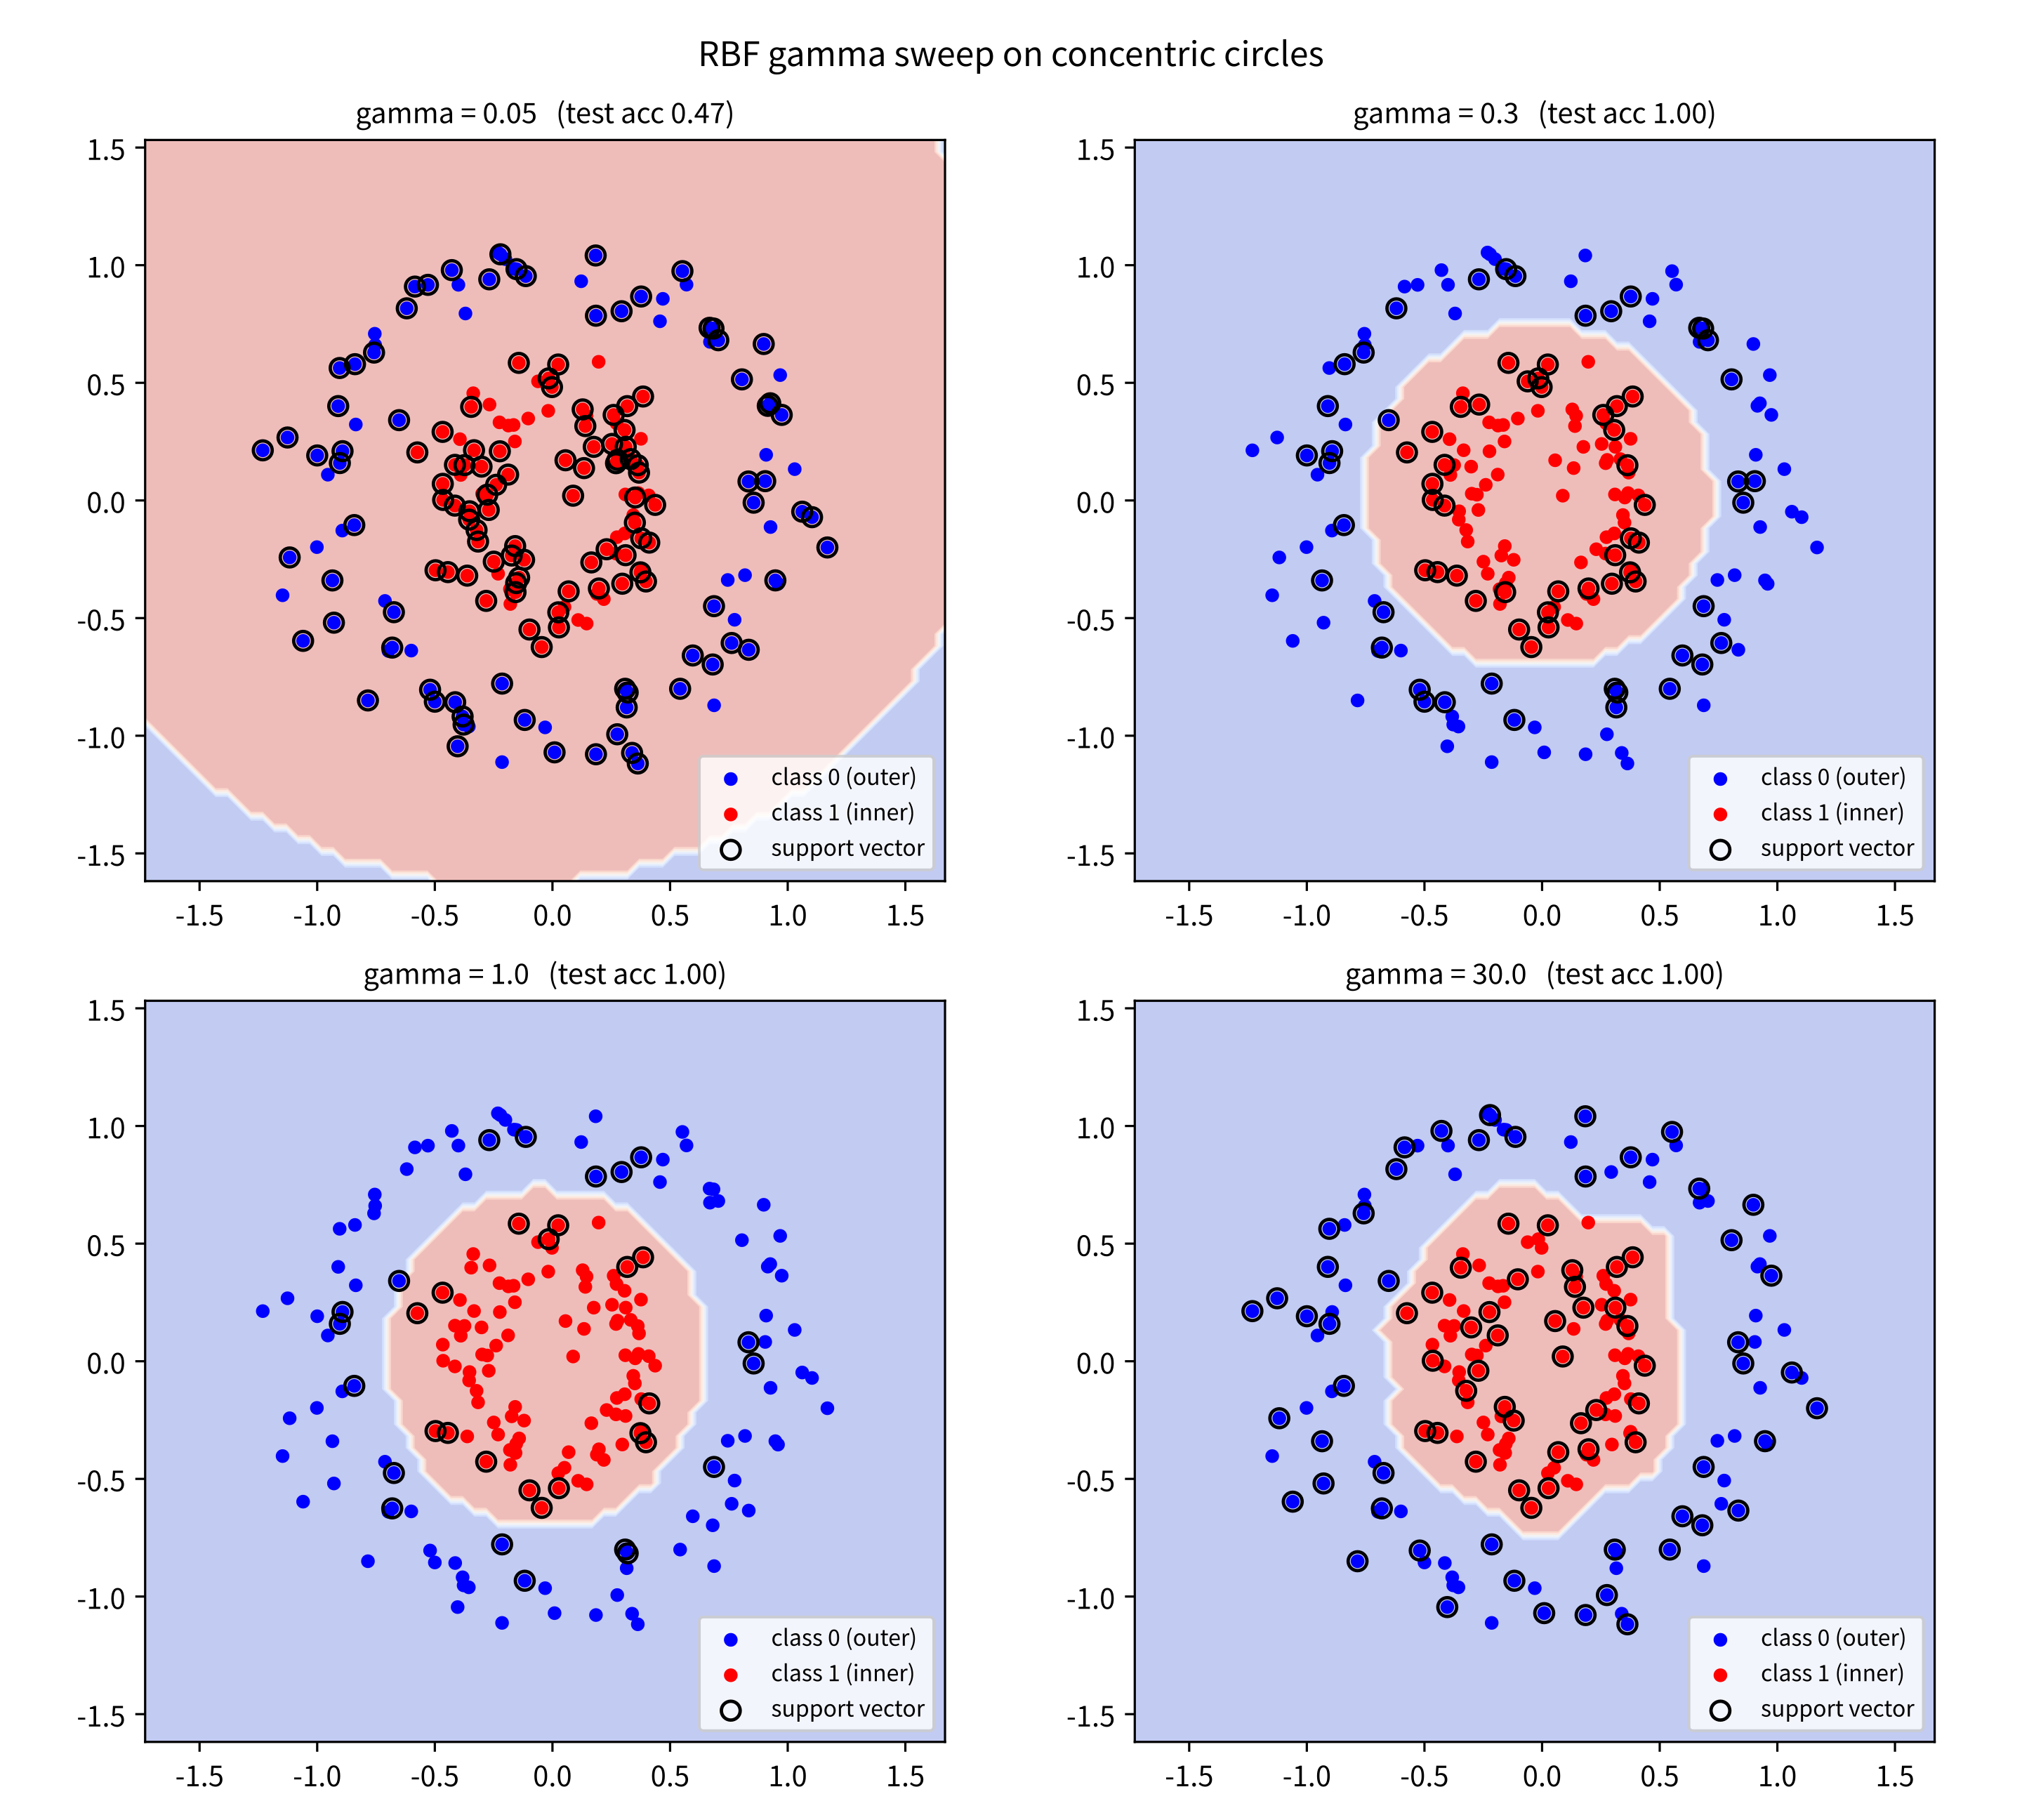
\includegraphics[width=\linewidth]{ch05_3_gamma_sweep.png}
    \end{column}
    \begin{column}{0.44\textwidth}
      \small
      \begin{itemize}
        \item $\gamma=0.05$: 거의 \textbf{직선}에 가까운 경계.
        \item $\gamma=1.0$: \textbf{원형}에 가깝게 수렴.
        \item $\gamma=30$: 점 하나하나를 감싸는 형태로
          \textbf{구불거림}.
      \end{itemize}
      \vskip0.4em
      \begin{block}{직관}
        커널 SVM의 예측 = ``새 점이 각 SV와 얼마나 비슷한가''
        (커널값)를 \textbf{가중 투표}.
        $\sigma$ 작음($\gamma$ 큼) $\Rightarrow$ 아주 가까운 SV만
        강하게 반영(복잡한 경계, 과적합 위험).
        $\sigma$ 큼($\gamma$ 작음) $\Rightarrow$ 멀리 있는 SV까지
        두루 반영(단순한 경계, 과소적합 위험).
      \end{block}
    \end{column}
  \end{columns}
\end{frame}

\begin{frame}[fragile]{실습: RBF 전개를 수치로 검증 — 교대 수렴}
  $\phi(x)$ 를 도수 합 $k\le N$ 으로 절단하고, 부분합의 내적이
  정확한 커널값 $K(x,x')$ 으로 수렴하는지:
  \begin{lstlisting}
def phi_terms(x, N):   # 도수 합 |alpha| <= N 인 모든 성분 phi_alpha(x)
    x1, x2 = x; out = []
    for a1 in range(N + 1):
        for a2 in range(N - a1 + 1):
            k = a1 + a2
            out.append(math.exp(-gamma * (x1*x1 + x2*x2))
                       * (2 * gamma) ** (k / 2) * x1 ** a1 * x2 ** a2
                       / (math.sqrt(math.factorial(a1))
                          * math.sqrt(math.factorial(a2))))
    return out
def rbf(x, z, g=gamma):
    return math.exp(-g * np.sum((np.asarray(x) - np.asarray(z)) ** 2))
x, z = (1.2, -0.7), (0.5, 1.1)
exact = rbf(x, z)
for N in [0, 1, 2, 5, 10, 20, 40]:
    s = sum(a * b for a, b in zip(phi_terms(x, N), phi_terms(z, N)))
    print(f"도수 합 <= {N:2d}: 부분합 = {s:.10f}   (오차 {s - exact:+.2e})")
\end{lstlisting}
  \vskip0.3em
  \small
  \begin{tabular}{@{}ccc@{}}
    \toprule
    $N$ (도수 절단) & 부분합 내적 & 오차 \\
    \midrule
    0 & 0.0337 & $+9.7\times10^{-3}$ \\
    1 & 0.0222 & $-1.8\times10^{-3}$ \\
    2 & 0.0242 & $+2.0\times10^{-4}$ \\
    5 & 0.02399 & $-6.9\times10^{-8}$ \\
    10 & 0.0239928358 & $\approx 0$ \\
    \bottomrule
  \end{tabular}
  \normalsize\vskip0.4em
  \begin{itemize}
    \item 정확한 값 $K(x,z) = 0.0239928358$.
    \item $N=0$: 0.0337로 \textbf{크고}, $N=1$: 0.0222로
      \textbf{작고}, $N=2$: 다시 초과, $N\ge5$에서 급격히 수렴 —
      테일러급수의 \textbf{교대 수렴}(oscillating convergence).
    \item $N=10$이면 오차 $10^{-15}$ 수준(이중 정밀도의 한계).
  \end{itemize}
  \vskip0.4em
  \begin{block}{핵심}
    $\phi$ 는 무한차원 벡터지만 \textbf{커널 SVM은 $\phi$ 를 직접
    계산하지 않는다} — 쌍대 문제의 구조가 그렇다. 실제로 계산하는
    것은 \textbf{커널값 $K(x,x')$ 뿐}이고, 그 값은 유클리드 거리
    하나로 계산된다. ``무한차원''은 $\phi$ 의 \textbf{개념적}
    차원일 뿐, \textbf{실제 계산 비용이 무한하다는 뜻이 아니다}.
  \end{block}
\end{frame}

\begin{frame}[fragile]{실습: 다항 커널로 XOR 분류}
  \begin{lstlisting}
def phi2(x):
    # (x.x'+1)^2 를 도수 2 이하 단항식으로 전개하면 6개의 성분이 필요하다:
    # x1^2, x2^2, 2*x1*x2 (-> sqrt2 계수), 2*x1, 2*x2 (-> sqrt2 계수), 1
    x1, x2 = x
    s2 = math.sqrt(2)
    return np.array([x1 ** 2, x2 ** 2, s2 * x1 * x2, s2 * x1, s2 * x2, 1.0])

# 커널값과 명시적 내적이 일치하는지 확인 (커널 트릭의 "같은 내적")
rng = np.random.default_rng(0)
Xs = rng.normal(size=(50, 2))
P = np.array([phi2(x) for x in Xs])
K_poly = ((Xs @ Xs.T + 1) ** 2)                    # (x.x' + 1)^2
K_exp  = P @ P.T                                   # phi2(x).phi2(x')
print("max |K_poly - K_explicit| =", np.max(np.abs(K_poly - K_exp)))
assert np.max(np.abs(K_poly - K_exp)) < 1e-10
print("일치: (x.x'+1)^2 는 정확히 phi2의 내적이다")

# XOR 사분면 데이터: y = -sign(x1*x2), 4개 사분면 클러스터
rng2 = np.random.default_rng(3)
n = 80
quads  = np.array([[ 1,  1], [ 1, -1], [-1,  1], [-1, -1]])
labels = np.array([-1, 1, 1, -1])
Xq = np.vstack([rng2.normal(q * 3, 0.8, (n, 2)) for q in quads])
yq = np.repeat(labels, n)
perm = rng2.permutation(len(yq)); Xq, yq = Xq[perm], yq[perm]
# d=1 (linear) vs d=2 (poly, degree=2, coef0=1) 학습 + 정확도 출력
\end{lstlisting}
\end{frame}

\begin{frame}{커널 트릭의 직접 검증 + XOR 결과}
  \begin{itemize}
    \item \kb{커널 트릭 직접 검증}: $\phi_2$ 의 내적이 정확히
      $(x\cdot x'+1)^2$ 와 같은지 50개 랜덤 점으로 확인 —
      최대 오차 $10^{-14}$ 수준으로 \textbf{숫자 하나까지 일치}.
      ``커널 트릭은 전개를 생략할 뿐, 같은 내적을 계산한다''의
      직접 검증.
  \end{itemize}
  \vskip0.5em
  \small
  \begin{tabular}{@{}lccc@{}}
    \toprule
    모델 & 정확도 & 서포트 벡터 수 & 비고 \\
    \midrule
    선형 (d=1) & 0.74 & 319 & 대각선 교차를 못 나눔 \\
    다항 d=2 & \textbf{1.00} & 18 & $x_1x_2$ 항 포함 \\
    \bottomrule
  \end{tabular}
  \normalsize\vskip0.4em
  \begin{columns}[T]
    \begin{column}{0.52\textwidth}
      \centering
      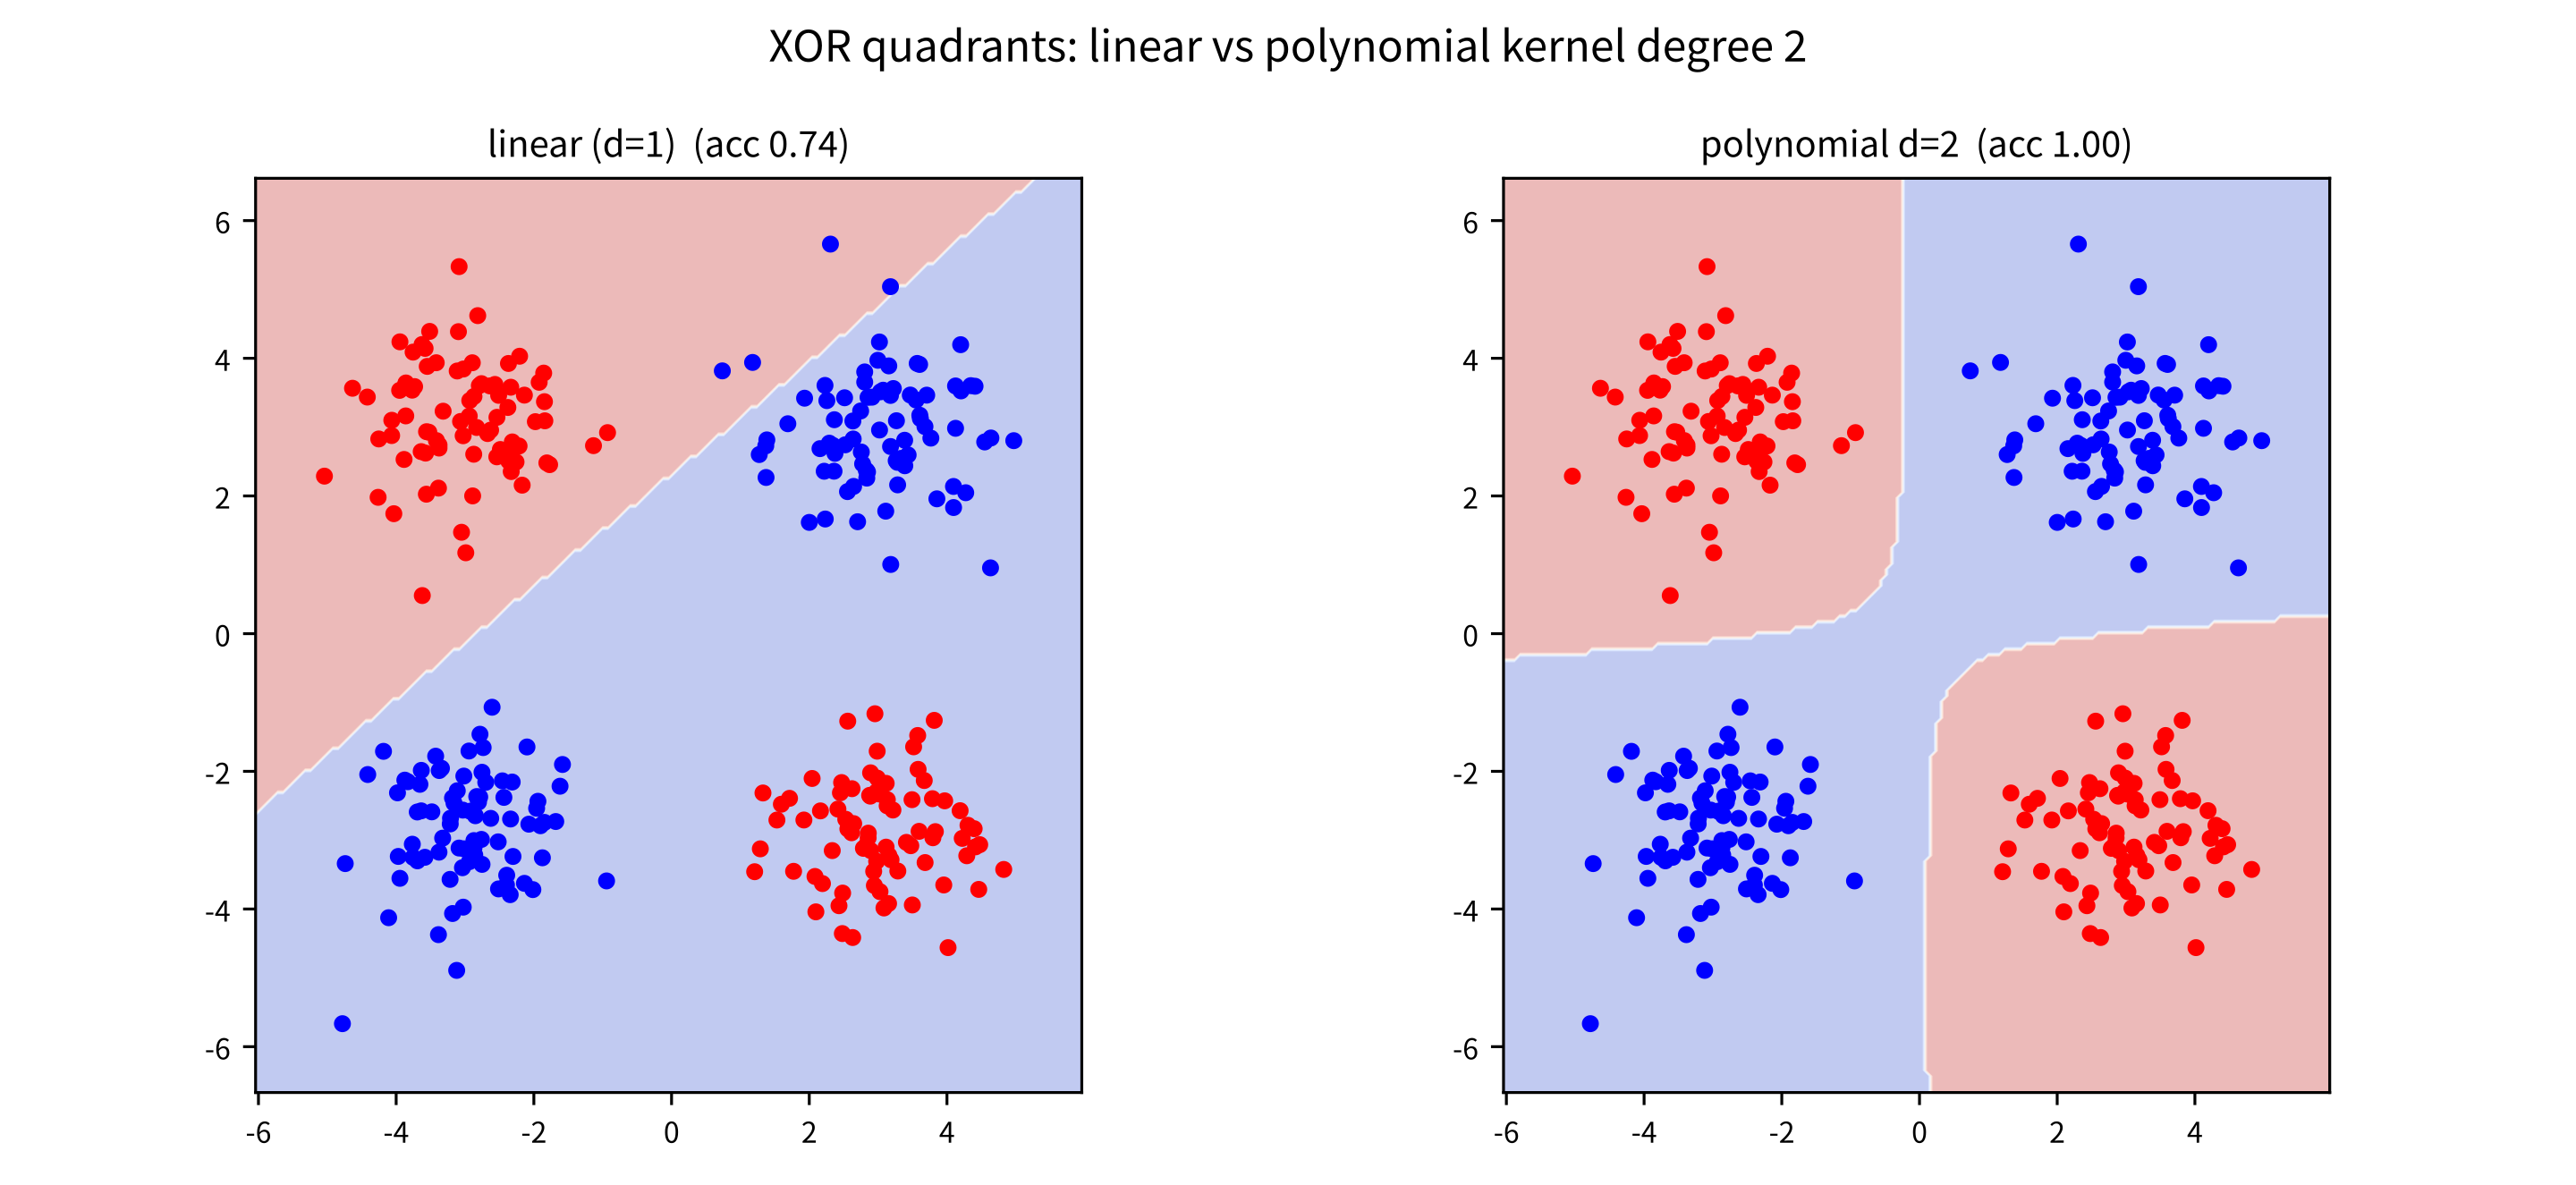
\includegraphics[width=\linewidth]{ch05_3_poly_xor.png}
    \end{column}
    \begin{column}{0.44\textwidth}
      \small
      \begin{itemize}
        \item \textbf{도수 하나만 바꿨을 뿐}인데 SV가
          319$\to$18로 줄고 정확도 0.74$\to$1.00.
        \item 선형(좌): 원점을 지나는 직선 하나에 머물며
          대각선 교차를 못 나눔.
        \item d=2(우): 경계가 \textbf{쌍곡선형}
          ($x_1x_2=c$ 곡선)으로 사분면을 따라 구부러짐 —
          ``도수 2 단항식 $x_1x_2$ 가 추가된'' 효과의 시각화.
      \end{itemize}
    \end{column}
  \end{columns}
\end{frame}

\begin{frame}{자주 하는 실수: $\gamma$ 를 ``느낌''으로 고르기}
  \begin{itemize}
    \item \texttt{gamma}(대략 $\frac{1}{2\sigma^2}$)가 ``결정
      경계가 얼마나 구불구불해질 수 있는가''를 \textbf{통째로}
      결정.
    \item \kb{$\gamma$ 극단적으로 크게}($\sigma$ 작음): 각 학습점
      바로 주변에 좁고 뾰족한 ``영향권'' $\Rightarrow$ 학습 데이터
      하나하나를 거의 다 따로 감싸는 \textbf{심하게 구불거림}
      (전형적 \textbf{과적합}).
    \item \kb{$\gamma$ 너무 작게}: 모든 점의 영향권이 서로 겹쳐
      사실상 \textbf{선형 커널과 비슷}하게 뭉뚱그려진 경계만
      나옴(과소적합).
  \end{itemize}
  \vskip0.4em
  \begin{block}{수치적 증거: 앞 $\gamma$ 스윕 표}
    $\gamma=0.05$: test 0.467로 \textbf{동전 던지기보다 나쁨}(선형
    0.517보다도 낮음) — RBF가 ``거의 상수 행렬''에 가까워져
    ``모든 점이 비슷'' $\Rightarrow$ 사실상 \textbf{무작위}.
    $\gamma=30$: train/test 1.00 — \textbf{이 데이터는 노이즈가
    적어} 운 좋게 일반화되는 것. 노이즈 있는 실전 데이터에선
    개별 노이즈 패턴까지 따라붙어 test가 \textbf{급락}.
  \end{block}
  \vskip0.4em
  {\footnotesize 4.1절 kNN의 $k$, 5.2절의 $C$와 \textbf{같은 종류}의
  ``복잡도 손잡이'' — $C$와 $\gamma$ 를 \textbf{동시에} 그리드
  서치하는 것이 표준(서로 영향을 주고받음).}
  \vskip0.3em
  \begin{center}
  \kq{검증셋으로 $(C, \gamma)$ 를 함께 그리드 서치하는 것 =\\
      5.2절 $C$ 튜닝의 비선형 버전.}
  \end{center}
\end{frame}

\begin{frame}{유명한 사례: 딥러닝 이전 시대, 우편번호를 읽던 SVM}
  \begin{itemize}
    \item 1990년대 미국 우편 서비스(USPS)는 \textbf{손으로 쓴
      우편번호}를 자동으로 읽어내는 문제로 골머리를 앓았다.
    \item 초기 신경망(LeCun의 CNN 포함)과 나란히 가장 강력한
      성능을 보인 방법 중 하나가 바로 \textbf{RBF 커널 SVM} —
      필기체 숫자처럼 명확한 직선으로 나뉘지 않는 복잡한 패턴에서도
      오차율을 \textbf{한 자릿수 퍼센트대}까지 끌어내림.
    \item 2010년대 초반 딥러닝(특히 10장 CNN, Krizhevsky et al.
      2012)이 대세가 되기 전까지 커널 SVM은 이미지 인식부터
      텍스트 분류(스팸 필터링에도 나이브베이즈와 나란히),
      생물정보학의 유전자 데이터 분류까지 폭넓게 쓰인
      ``\textbf{만능 분류기}''.
  \end{itemize}
  \vskip0.5em
  \begin{block}{지금도}
    데이터가 \textbf{수천$\sim$수만 개 수준}으로 많지 않고 특징 수가
    적당할 때는, 신경망보다 \textbf{학습이 훨씬 빠르고
    하이퍼파라미터도 적은} 커널 SVM이 실무에서 여전히 합리적인
    선택지.
  \end{block}
\end{frame}

\begin{frame}{이 절의 핵심 세 가지}
  \begin{block}{SVM = 같은 문제, 다른 원칙}
    로지스틱회귀·GDA와 \textbf{같은 문제}(선형 결정 경계)를
    ``\textbf{마진을 최대화한다}''는 다른 원칙으로 풀고 —
    \textbf{원칙이 다르면 얻는 성질(서포트 벡터, 커널 트릭)도
    달라진다.}
  \end{block}
  \vskip0.4em
  \begin{enumerate}
    \item \kb{고차원 = ``휘어진 경계''를 ``평평한 경계''로}:
      원형 데이터는 $z=x_1^2+x_2^2$ 축을 추가하면 두 수평 고도로
      벌어져 평면 하나로 잘림. XOR은 $x_1x_2$ 축이 필요.
    \item \kb{커널 트릭 = ``내적만 계산하자'':} 쌍대 문제에서
      데이터는 $\phi(x^{(i)})\cdot\phi(x^{(j)})$ 로만 등장하므로,
      이 내적값을 $K(x,x')$ 으로 교체해도 해가 변하지 않음.
      2$\times$2 커널 행렬 예제로 primal과 dual이 같은 해
      ($w=(1/6,1/6)$)을 줌을 확인.
    \item \kb{$\gamma$(또는 다항 커널의 도수 $d$)는 ``경계의
      구불 복잡도'' 손잡이}: $\gamma$ 가 작으면 직선(과소적합),
      크면 점마다 봉우리(과적합). \textbf{반드시 $(C,\gamma)$ 를
      함께 검증셋으로 튜닝}.
  \end{enumerate}
  \vskip0.6em
  \begin{block}{6장(정규화와 모델 선택)으로 넘어가기 전, 연결고리}
    이번 절의 $C$, $\gamma$ 튜닝은 6장의 \textbf{교차 검증}으로
    체계화 — 검증셋 정확도로 $(C,\gamma)$ 를 함께 그리드 서치가
    표준 관행.
    10장(신경망)에서 RBF의 ``봉우리''와 CNN의 \textbf{커널 필터}는
    수학적으로 다른 개념이지만, ``원본 특징을 고차 항으로 변환해
    선형 분류''한다는 큰 그림은 이어진다.
  \end{block}
\end{frame}

\begin{frame}{자주 묻는 질문}
  \small
  \textbf{Q. 커널을 아무 함수나 써도 되나요?}
  \begin{itemize}
    \item 아니다 — 어떤 $\phi$ 의 내적에 대응하려면 \kb{머서 조건}
      (커널 행렬이 \textbf{양의 준정부호})을 만족해야 함.
      다항·RBF는 증명되어 안심하고 쓸 수 있지만, 아무 함수는
      안 된다.
  \end{itemize}
  \vskip0.4em
  \textbf{Q. $\phi$ 가 무한차원이면 어떻게 학습하나요?}
  \begin{itemize}
    \item $\phi$ 자체를 \textbf{계산하지 않기 때문에} — 쌍대 문제
      구조상 데이터는 \textbf{내적값}으로만 등장하고, RBF는
      유클리드 거리 하나로 계산.
    \item ``무한차원''은 \textbf{개념적} 차원일 뿐, 실제 계산
      비용이 무한하다는 뜻이 \textbf{아님}.
  \end{itemize}
  \vskip0.4em
  \textbf{Q. 다항 커널의 도수 $d$ 는 어떻게 고르나요?}
  \begin{itemize}
    \item $d$ 는 ``경계가 얼마나 복잡한 곡면일 수 있는가'' 조절 —
      $d=1$ 직선, $d=2$ 포물선/쌍곡선형, $d=3$ 더 복잡한 곡면.
      \textbf{$d$ 를 키울수록 과적합 위험}.
      XOR에선 $d=2$가 정확히 필요했지만, 실전은 \textbf{검증셋으로
      튜닝}($(C,d)$ 함께 그리드 서치, $d>3$은 거의 안 씀).
  \end{itemize}
  \vskip0.4em
  {\footnotesize 이 ``내적만 계산하면 고차원 변환을 우회한다''는
  원리는 SVM에만 국한 \textbf{아님} — RBF 네트워크, Gaussian
  Processes, 신경망의 \textbf{커널 정리}(neural tangent kernel,
  Jacot et al. 2018)까지 이어진다.}
\end{frame}

% ===== wrap-up =====
\begin{frame}{이번 주차 정리}
  \small
  \begin{itemize}
    \item \textbf{5.1} \kb{마진 최대화 = $\|w\|$ 최소화} —
      스케일 불변성 때문에 제약 $y(w^\top x+b)\ge1$이 필수,
      마진 $2/\|w\|$, \kb{서포트 벡터}만 경계를 떠받침
      (로지스틱회귀의 ``모든 점 기여''와 대조).
    \item \textbf{5.2} \kb{소프트 마진} — 여유 변수 $\xi$ +
      \kb{힌지 손실}로 노이즈를 허용, $C$는 ``이상치 용인도''
      손잡이. 힌지의 \textbf{비활성화} 성질($f\ge1$에서 그래디언트
      0)이 SV 개념을 가능하게 함. $1/C$ $\Leftrightarrow$ 6장의
      정규화 세기 $\lambda$.
    \item \textbf{5.3} \kb{커널 트릭} — 고차원으로 휘어진 경계를
      평평하게, 쌍대 문제에서 \textbf{내적만} 계산하면 $\phi$ 의
      차원을 우회. RBF의 무한차원은 개념뿐, $m$개 데이터의 커널
      행렬 rank $\le m$. $\gamma$ (또는 도수 $d$)는 경계의 구불
      복잡도 —
      $(C,\gamma)$ 를 \textbf{함께} 검증셋으로 튜닝.
  \end{itemize}
  \vskip0.6em
  \begin{block}{다음 주차 --- Chapter 6. 정규화와 모델 선택}
    5.2절의 $C$가 ``마진을 넓게 잡을 것인가, 위반을 덜 허용할
    것인가''를 조절하는 손잡이라면, 6장은 이 ``충실도 vs
    단순함''의 손잡이를 \textbf{L1/L2 페널티와 교차검증}이라는
    일반 틀로 확장한다. SVM의 $C$ 튜닝이 바로 그 첫 번째
    사례다.
  \end{block}
\end{frame}

\end{document}
